\documentclass[letterpaper,oneside,11pt]{book}

%fonts related
\usepackage{helvet}
\renewcommand{\familydefault}{\sfdefault}
\usepackage{textcomp}

%spell related
\usepackage[spanish]{babel}
\usepackage[utf8]{inputenc}

%graphics related
\usepackage{adjustbox}
\usepackage{graphicx}
\usepackage{pstricks}

\usepackage{tikz}
\usetikzlibrary{trees}
\tikzstyle{every node}=[draw=black,thick,anchor=west]
\tikzstyle{form}=[draw=black,fill=yellow!20]
\tikzstyle{confirm}=[draw=black,fill=green!20]

\usepackage{graphicx}

\usepackage{listings}
\usepackage{longtable}
\usepackage{lscape}

%margin related
\usepackage{anysize}
\marginsize{3cm}{2cm}{2cm}{2cm}

\setlength{\parskip}{6pt}

\usepackage{rotating}
\usepackage{multirow}

\usepackage{fancyhdr}
\pagestyle{fancy}

\fancyhead[LE,RO]{\slshape}
\fancyhead[LO,RE]{\slshape \leftmark}

\usepackage[grey]{quotchap}

\usepackage[
pdfauthor={Carlos Eduardo Caballero Burgoa},%
pdftitle={Salesforce (Productos y Listas de Precios)},%
colorlinks,%
citecolor=black,%
filecolor=black,%
linkcolor=black,%
urlcolor=black
pdftex]{hyperref}

\newcommand{\blankpage}{
\newpage
\thispagestyle{empty}
\mbox{}
\newpage
}

\usepackage[nottoc,notlof,notlot]{tocbibind}
\usepackage{float}

\begin{document}
\frontmatter

\newcommand{\umsslogo}{
\adjustbox{valign=t}{%LaTeX with PSTricks extensions
%%Creator: inkscape 0.48.5
%%Please note this file requires PSTricks extensions
\psset{xunit=.5pt,yunit=.5pt,runit=.5pt}
\begin{pspicture}(128,128)
{
\newrgbcolor{curcolor}{0 0 0.50196081}
\pscustom[linestyle=none,fillstyle=solid,fillcolor=curcolor]
{
\newpath
\moveto(17.48167,126.01987)
\lineto(110.51833,126.01987)
\lineto(64,-0.84852)
\closepath
}
}
{
\newrgbcolor{curcolor}{1 1 1}
\pscustom[linestyle=none,fillstyle=solid,fillcolor=curcolor]
{
\newpath
\moveto(20,124.3535884)
\lineto(108,124.3515884)
\lineto(64,4.3534684)
\closepath
}
}
{
\newrgbcolor{curcolor}{1 0 0}
\pscustom[linestyle=none,fillstyle=solid,fillcolor=curcolor]
{
\newpath
\moveto(20,124.3496821)
\lineto(37.601563,76.3496824)
\lineto(64,94.3512444)
\closepath
}
}
{
\newrgbcolor{curcolor}{1 0 0}
\pscustom[linestyle=none,fillstyle=solid,fillcolor=curcolor]
{
\newpath
\moveto(108,124.3516384)
\lineto(90.398437,76.3496784)
\lineto(64,94.3512484)
\closepath
}
}
{
\newrgbcolor{curcolor}{0 0 0.50196081}
\pscustom[linestyle=none,fillstyle=solid,fillcolor=curcolor]
{
\newpath
\moveto(41.46875,122.75001)
\lineto(41.46875,116.09375)
\curveto(41.46875,113.893366)(43.274007,112.125)(45.481289,112.125)
\lineto(47.456211,112.125)
\curveto(49.663493,112.125)(51.46875,113.893366)(51.46875,116.09375)
\lineto(51.46875,122.75001)
\lineto(48.020474,122.75001)
\lineto(48.020474,116.15625)
\curveto(48.020474,116.13515)(48.021316,116.11464)(48.020474,116.09375)
\curveto(47.987324,115.270476)(47.287066,114.625)(46.453076,114.625)
\curveto(45.619086,114.625)(44.950177,115.270476)(44.917026,116.09375)
\lineto(44.917026,116.15625)
\lineto(44.917026,122.75001)
\closepath
}
}
{
\newrgbcolor{curcolor}{0 0 0.50196081}
\pscustom[linestyle=none,fillstyle=solid,fillcolor=curcolor]
{
\newpath
\moveto(53.477982,122.75)
\lineto(53.477982,112.125)
\lineto(56.279043,112.125)
\lineto(56.279043,117.90625)
\lineto(57.912995,112.125)
\lineto(60.013791,112.125)
\lineto(61.676921,117.90625)
\lineto(61.676921,112.125)
\lineto(64.477982,112.125)
\lineto(64.477982,122.75)
\lineto(60.743234,122.75)
\lineto(58.963393,116.09375)
\lineto(57.21273,122.75)
\lineto(53.477982,122.75)
\closepath
}
}
{
\newrgbcolor{curcolor}{0 0 0.50196081}
\pscustom[linestyle=none,fillstyle=solid,fillcolor=curcolor]
{
\newpath
\moveto(67.80744,121.7794318)
\curveto(69.565499,123.0541348)(72.415875,123.0541348)(74.173934,121.7794318)
\curveto(75.018184,121.1672978)(75.492479,120.337066)(75.48546,119.4713779)
\lineto(72.182288,119.4713778)
\curveto(72.182288,119.980539)(71.64879,120.3251893)(70.990687,120.3251893)
\curveto(70.332585,120.3251893)(69.745027,119.9082237)(69.807016,119.4759072)
\curveto(69.854566,119.1443138)(70.491901,118.9300671)(72.004371,118.5803762)
\curveto(73.49381,118.2360104)(74.180395,117.687588)(74.180395,117.687588)
\curveto(75.925051,116.420155)(75.925051,114.353453)(74.166985,113.07875)
\curveto(72.408926,111.804047)(69.55855,111.804047)(67.800491,113.07875)
\curveto(66.956241,113.690884)(66.481946,114.521116)(66.488965,115.386804)
\lineto(69.792137,115.386804)
\curveto(69.792137,114.877643)(70.325635,114.532993)(70.983737,114.532993)
\curveto(71.64184,114.532993)(72.229398,114.949958)(72.167409,115.382275)
\curveto(72.119859,115.713868)(71.40474,115.989855)(69.970054,116.277806)
\curveto(68.62588,116.547589)(67.794032,117.170595)(67.794032,117.170595)
\curveto(66.049378,118.4380269)(66.049378,120.5047288)(67.807442,121.7794318)
\closepath
}
}
{
\newrgbcolor{curcolor}{0 0 0.50196081}
\pscustom[linestyle=none,fillstyle=solid,fillcolor=curcolor]
{
\newpath
\moveto(78.816672,121.7794318)
\curveto(80.574731,123.0541348)(83.425107,123.0541348)(85.183166,121.7794318)
\curveto(86.027416,121.1672978)(86.501711,120.337066)(86.494692,119.4713779)
\lineto(83.19152,119.4713778)
\curveto(83.19152,119.980539)(82.658022,120.3251893)(81.999919,120.3251893)
\curveto(81.341817,120.3251893)(80.754259,119.9082237)(80.816248,119.4759072)
\curveto(80.863798,119.1443138)(81.501133,118.9300671)(83.013603,118.5803762)
\curveto(84.503042,118.2360104)(85.189627,117.687588)(85.189627,117.687588)
\curveto(86.934283,116.420155)(86.934283,114.353453)(85.176217,113.07875)
\curveto(83.418158,111.804047)(80.567782,111.804047)(78.809723,113.07875)
\curveto(77.965473,113.690884)(77.491178,114.521116)(77.498197,115.386804)
\lineto(80.801369,115.386804)
\curveto(80.801369,114.877643)(81.334867,114.532993)(81.992969,114.532993)
\curveto(82.651072,114.532993)(83.23863,114.949958)(83.176641,115.382275)
\curveto(83.129091,115.713868)(82.413972,115.989855)(80.979286,116.277806)
\curveto(79.635112,116.547589)(78.803264,117.170595)(78.803264,117.170595)
\curveto(77.05861,118.4380269)(77.05861,120.5047288)(78.816674,121.7794318)
\closepath
}
}
{
\newrgbcolor{curcolor}{1 1 1}
\pscustom[linestyle=none,fillstyle=solid,fillcolor=curcolor]
{
\newpath
\moveto(70.14999998,76.37293303)
\curveto(70.14999998,72.9763818)(67.39655118,70.222933)(63.99999996,70.222933)
\curveto(60.60344874,70.222933)(57.84999994,72.9763818)(57.84999994,76.37293303)
\curveto(57.84999994,79.76948425)(60.60344874,82.52293305)(63.99999996,82.52293305)
\curveto(67.39655118,82.52293305)(70.14999998,79.76948425)(70.14999998,76.37293303)
}
}
{
\newrgbcolor{curcolor}{0 0 0.50196081}
\pscustom[linewidth=0.75000002,linecolor=curcolor]
{
\newpath
\moveto(68.71231739,82.86972446)
\lineto(59.24350298,82.84649785)
\lineto(56.33956823,73.83394278)
\lineto(64.01365227,68.28710404)
\lineto(71.66043178,73.87152423)
\closepath
}
}
{
\newrgbcolor{curcolor}{0 0 0.50196081}
\pscustom[linewidth=0.75000002,linecolor=curcolor]
{
\newpath
\moveto(67.99473993,81.84342952)
\lineto(63.9999999,78.90862405)
\lineto(59.99782385,81.84689855)
\lineto(61.55454715,77.14077025)
\lineto(57.52334163,74.24245139)
\lineto(62.48018957,74.26870961)
\lineto(63.9909436,69.53917555)
\lineto(65.4977208,74.26153231)
\lineto(70.46262365,74.23683838)
\lineto(66.43701524,77.12915715)
\closepath
}
}
{
\newrgbcolor{curcolor}{0 0 0.50196081}
\pscustom[linewidth=0.23791535,linecolor=curcolor]
{
\newpath
\moveto(65.53953053,74.20499964)
\lineto(62.44603561,74.21258785)
\lineto(61.49730993,77.15702124)
\lineto(64.00446014,78.96919294)
\lineto(66.50268986,77.14474325)
\closepath
}
}
{
\newrgbcolor{curcolor}{0 0 0.50196081}
\pscustom[linewidth=0.75,linecolor=curcolor]
{
\newpath
\moveto(56.902008,46.063218)
\lineto(71.745005,73.889359)
}
}
{
\newrgbcolor{curcolor}{0 0 0.50196081}
\pscustom[linewidth=0.75,linecolor=curcolor]
{
\newpath
\moveto(71.072435,46.164257)
\lineto(56.249925,73.865129)
}
}
{
\newrgbcolor{curcolor}{0 0 0.50196081}
\pscustom[linewidth=0.75,linecolor=curcolor]
{
\newpath
\moveto(64,28.218365)
\lineto(64,68.311947)
}
}
{
\newrgbcolor{curcolor}{0 0 0.50196081}
\pscustom[linestyle=none,fillstyle=solid,fillcolor=curcolor]
{
\newpath
\moveto(62.483156,28.843501)
\curveto(63.607731,28.523615)(64.380752,28.537068)(65.516844,28.843501)
\curveto(64.862934,27.58287)(64.579942,27.6015)(64.008692,26.04245)
\curveto(63.419763,27.6257)(63.145632,27.60857)(62.483156,28.843501)
\closepath
}
}
{
\newrgbcolor{curcolor}{0 0 0.50196081}
\pscustom[linestyle=none,fillstyle=solid,fillcolor=curcolor]
{
\newpath
\moveto(69.288692,46.076591)
\curveto(70.422546,46.361849)(71.085275,46.760011)(71.915943,47.593435)
\curveto(71.979953,46.174742)(71.725563,46.04938)(72.010373,44.413578)
\curveto(70.708721,45.490248)(70.479882,45.338348)(69.288695,46.076591)
\closepath
}
}
{
\newrgbcolor{curcolor}{0 0 0.50196081}
\pscustom[linestyle=none,fillstyle=solid,fillcolor=curcolor]
{
\newpath
\moveto(58.726361,46.076591)
\curveto(57.592507,46.361849)(56.929778,46.760011)(56.09911,47.593435)
\curveto(56.0351,46.174742)(56.28949,46.04938)(56.00468,44.413578)
\curveto(57.306332,45.490248)(57.535171,45.338348)(58.726358,46.076591)
\closepath
}
}
\end{pspicture}
}
}
\newcommand{\fcytlogo}{
\adjustbox{valign=t}{%LaTeX with PSTricks extensions
%%Creator: inkscape 0.48.5
%%Please note this file requires PSTricks extensions
\psset{xunit=.5pt,yunit=.5pt,runit=.5pt}
\begin{pspicture}(128,128)
{
\newrgbcolor{curcolor}{1 0.18431373 0.02352941}
\pscustom[linestyle=none,fillstyle=solid,fillcolor=curcolor]
{
\newpath
\moveto(12.60317454,12.35940966)
\lineto(12.60317454,115.6405906)
\lineto(115.3968244,115.6405906)
\lineto(115.3968244,106.72423025)
\lineto(20.94189438,106.72423025)
\lineto(20.94189438,64.18575417)
\lineto(58.2387053,64.18575417)
\lineto(58.2387053,55.67805896)
\lineto(20.94189438,55.67805896)
\lineto(20.94189438,12.35940966)
\closepath
}
}
{
\newrgbcolor{curcolor}{0 0 0}
\pscustom[linewidth=0.89156044,linecolor=curcolor]
{
\newpath
\moveto(12.60317454,12.35940966)
\lineto(12.60317454,115.6405906)
\lineto(115.3968244,115.6405906)
\lineto(115.3968244,106.72423025)
\lineto(20.94189438,106.72423025)
\lineto(20.94189438,64.18575417)
\lineto(58.2387053,64.18575417)
\lineto(58.2387053,55.67805896)
\lineto(20.94189438,55.67805896)
\lineto(20.94189438,12.35940966)
\closepath
}
}
{
\newrgbcolor{curcolor}{1 0.18431373 0.02352941}
\pscustom[linestyle=none,fillstyle=solid,fillcolor=curcolor]
{
\newpath
\moveto(28.74996694,73.06496267)
\lineto(28.74996694,98.17938319)
\lineto(115.3968244,98.17938319)
\lineto(115.3968244,89.48592873)
\lineto(38.52900646,89.48592873)
\lineto(38.52900646,81.60980974)
\lineto(115.3968244,81.60980974)
\lineto(115.3968244,73.06496267)
\closepath
}
}
{
\newrgbcolor{curcolor}{0 0 0}
\pscustom[linewidth=0.89156044,linecolor=curcolor]
{
\newpath
\moveto(28.74996694,73.06496267)
\lineto(28.74996694,98.17938319)
\lineto(115.3968244,98.17938319)
\lineto(115.3968244,89.48592873)
\lineto(38.52900646,89.48592873)
\lineto(38.52900646,81.60980974)
\lineto(115.3968244,81.60980974)
\lineto(115.3968244,73.06496267)
\closepath
}
}
{
\newrgbcolor{curcolor}{1 0.18431373 0.02352941}
\pscustom[linestyle=none,fillstyle=solid,fillcolor=curcolor]
{
\newpath
\moveto(65.97097162,64.18575417)
\lineto(115.3968244,64.18575417)
\lineto(115.3968244,55.67805896)
\lineto(74.1580759,55.67805896)
\lineto(74.1580759,46.9846097)
\lineto(115.3968244,46.9846097)
\lineto(115.3968244,38.06824935)
\lineto(28.7499659,38.06824935)
\lineto(28.7499659,46.9846097)
\lineto(65.97097162,46.9846097)
\closepath
}
}
{
\newrgbcolor{curcolor}{0 0 0}
\pscustom[linewidth=0.89156044,linecolor=curcolor]
{
\newpath
\moveto(65.97097162,64.18575417)
\lineto(115.3968244,64.18575417)
\lineto(115.3968244,55.67805896)
\lineto(74.1580759,55.67805896)
\lineto(74.1580759,46.9846097)
\lineto(115.3968244,46.9846097)
\lineto(115.3968244,38.06824935)
\lineto(28.7499659,38.06824935)
\lineto(28.7499659,46.9846097)
\lineto(65.97097162,46.9846097)
\closepath
}
}
{
\newrgbcolor{curcolor}{1 0.18431373 0.02352941}
\pscustom[linestyle=none,fillstyle=solid,fillcolor=curcolor]
{
\newpath
\moveto(28.7499659,29.67202527)
\lineto(115.3968244,29.67202527)
\lineto(115.3968244,21.27574922)
\lineto(74.1580759,21.27574922)
\lineto(74.1580759,12.35940966)
\lineto(65.97097162,12.35940966)
\lineto(65.97097162,21.27574922)
\lineto(28.7499659,21.27574922)
\closepath
}
}
{
\newrgbcolor{curcolor}{0 0 0}
\pscustom[linewidth=0.89156044,linecolor=curcolor]
{
\newpath
\moveto(28.7499659,29.67202527)
\lineto(115.3968244,29.67202527)
\lineto(115.3968244,21.27574922)
\lineto(74.1580759,21.27574922)
\lineto(74.1580759,12.35940966)
\lineto(65.97097162,12.35940966)
\lineto(65.97097162,21.27574922)
\lineto(28.7499659,21.27574922)
\closepath
}
}
\end{pspicture}
}
}

\begin{titlepage}

\begin{tabular}[t]{c p{8.6cm} c}
\umsslogo &
\vfill
\large{\textsc{Universidad Mayor de San Simón}} \newline
\large{\textsc{Facultad de Ciencias y Tecnología}} \newline
\large{\textsc{Carrera de Ingeniería de Sistemas}} &
\fcytlogo \\
\end{tabular}
\vfill
\begin{center}
\huge{\bf{Automatización de las pruebas de interfaz de usuario en Salesforce\\
Módulo de Productos y Listas de Precios}}
\end{center}
\vfill
\begin{tabbing}
\hspace{4cm}\=\+
\textbf{Modalidad:} Diplomado de Doble Titulación\\
\\
\textbf{Elaborado por:} Carlos Eduardo Caballero Burgoa\\
\\
%\textbf{Tutor:} \\
%\\
\end{tabbing}
\begin{center}
Cochabamba - Bolivia
\end{center}
\end{titlepage}


\blankpage

\tableofcontents
\listoffigures
\listoftables

\mainmatter
\chapter{Introducción}

Hoy en día muchas empresas de software, siguen procedimientos de desarrollo
ágiles, acelerando la producción y publicación de productos hacia el mercado;
esto presenta un gran reto tanto desde la perspectiva del aseguramiento de la
calidad del producto, como del seguimiento y control de la corrección de
errores.

La clave para agilizar estos procesos parte por optimizar y automatizar los
procesos de despliegue y evaluación del software, el cambio es necesario para
el manejo de proyectos de desarrollo grandes, o proyectos que siguen
lineamientos o estándares de cumplimiento muy estrictos.

Este capítulo define el propósito del presente trabajo, los antecedentes, los
objetivos, los alcances, y los factores que despertaron el interés por
resolverlos.

\section{Antecedentes}
\emph{Salesforce} es un servicio que apoya a la gestión de todo el flujo de
clientes que se tienen en una empresa, este tipo de software es conocido como
\emph{CRM}, y la meta principal es ayudar a gestionar las relaciones con los
clientes, además de conocer su necesidades y preferencias.

\emph{Salesforce} es el líder mundial como proveedor de su sistema \emph{CRM},
tanto para ventas, como servicio al cliente y mercadotecnia, por lo que es
necesario que provean a sus clientes de un software robusto y confiable.

Entre los muchos componentes que integran este servicio, uno de los elementos
básicos es aquel que gestiona los productos y las listas de precios. El módulo
de productos provee las funcionalidad de gestión para el catálogo de
los elementos que pueden comercializarse, mientras que el módulo de listas de
precios permite crear conjuntos personalizados de productos con precios de
lista asociados para usos específicos; ambos módulos estrechamente vinculados
entre si, y que son piezas fundamentales para otros componentes dentro del
sistema.

Garantizar el éxito del servicio implica tener un proceso de evaluación y
mejora continua del producto, haciendo que aquellos procesos repetitivos sean
automatizados y encaminados a cubrir aquellos criterios de calidad que
verdaderamente aporten valor al cliente.

\section{Definición del problema}
Siendo el módulo de productos y listas de precios componentes participes en la
funcionalidad provista por otros módulos de \emph{Salesforce}, un potencial
error en este podría tener un efecto en cascada con el potencial de afectar el
servicio completo, es por esta razón que es necesario priorizar la evaluación
de las funcionalidades disponibles por estos módulos.

\emph{Salesforce} sigue un política de actualizaciones muy continua, pudiendo
existir hasta tres versiones por año, lo que sin una automatización correcta
de las pruebas de interfaz de usuario, implicaría un enorme gasto de recursos
para la compañía.

Por lo mencionado se define el problema como:

\emph{«Garantizar la calidad de los elementos que componen la interfaz de
usuario requiere de un proceso de evaluación continuada y eficiente, de forma
que los módulos evaluados y sus diferentes versiones contengan la menor
cantidad posible de errores.»}.

\section{Objetivos}

\subsection{Objetivo General}
Implementar un \emph{framework} para la automatización de las pruebas de interfaz de
usuario en el módulo de Productos y Listas de Precios en \emph{Salesforce},
para garantizar un procedimiento continuo de evaluación y minimizar la cantidad
de errores que contiene el software.

\subsection{Objetivos Específicos}
\begin{itemize}
\item Formular los casos de prueba necesarios que los módulos de gestión de
    productos y listas de precios requieran para cubrir los atributos de calidad
    requeridos.
\item Diseñar e implementar los modelos y bibliotecas de funciones que
    conforman un \emph{framework} de automatización.
\item Automatizar los casos de prueba de las funciones que componen la interfaz
    de usuario del módulo de gestión de productos y listas de precios.
\end{itemize}

\section{Justificación}
Hoy en día, la automatización de pruebas es una tarea esencial para proporcionar
un servicio de evaluación de calidad adecuado, ya que los sistemas han crecido
tanto en tamaño como en complejidad.

Con una estrategia de automatización implementada apropiadamente el tiempo de
evaluar las nuevas funcionalidades del sistema, además de la evaluación de las
funcionalidades antiguas será reducido drásticamente, consiguiendo mejorar la
cobertura de las pruebas, junto con los beneficios propios de la automatización
\parencite{Software}.

\section{Alcance}
El proyecto cubrirá exclusivamente los componentes de interfaz del módulo de
productos y listas de precios, sin considerar aquellas funcionalidades dentro de
estos que requieran la utilización de otros módulos, de esta forma no se tomarán
en cuenta los siguientes aspectos:

\begin{itemize}
\item Generación de gráficas dentro de los módulos a evaluar.
\item Configuración de múltiples familias de productos.
\item Gestión de permisos de visibilidad de los elementos hacia diversas
    categorías de usuarios.
\item Evaluación y cumplimiento de los permisos de usuarios anteriormente
    citados.
\end{itemize}

Con respecto al proceso de desarrollo del \emph{framework}, se omitirá la
realización de pruebas unitarias, para reducir el tiempo de desarrollo y evitar
la necesidad de mantener las pruebas unitarias, además de mantener el
\emph{framework} propiamente dicho.


\chapter{Conceptos y Definiciones}

\section{Automatización de pruebas}
La automatización de pruebas es una técnica usada en aplicaciones para
implementar todo el ciclo de vida del software en menor tiempo, y proveyendo a
este proceso de eficiencia y efectividad en su etapa de evaluación.

La automatización de las pruebas es mas útil en el lanzamiento de nuevas
versiones de software, para evaluar que todos los errores anteriormente
corregidos no sean introducidos nuevamente, mientras que será difícil y costoso
hacer las pruebas manualmente, ejecutar las pruebas automatizadas será mas
efectivo en términos de costo, uso de los recursos, y aprovechamiento del
tiempo.

Se conoce que en los siguientes escenarios es útil automatizar:

\begin{itemize}
    \item Los requerimientos no cambian frecuentemente.
    \item Se accede al aplicativo con múltiples y variados usuarios, roles y
        privilegios.
    \item El software es estable respecto a sus pruebas manuales.
    \item Se cuenta con el tiempo necesario para automatización en el proyecto.
    \item El proyecto sigue o debe seguir estándares estrictos.
    \item La complejidad del proyecto es elevada.
    \item El proyecto requiere constantes revisiones en algunas de sus
    características.
\end{itemize}

\subsection{Criterios a seguir}
Existen muchas herramientas útiles para escribir rutinas de automatización, pero
los pasos identificables en el proceso pueden simplificarse en los siguientes:

\begin{itemize}
    \item Identificar áreas dentro del software para automatizar.
    \item Elegir la herramienta adecuada para la automatización.
    \item Escribir las rutinas de prueba.
    \item Desarrollar el conjunto de casos de prueba.
    \item Ejecutar los casos de prueba.
    \item Generar los reportes de resultados.
    \item Encontrar los posibles errores o aspectos negativos.
\end{itemize}

\subsection{Beneficios}
Los beneficios de implementar un proceso de automatización de pruebas son
diversos, entre los cuales destacan:

\begin{itemize}
    \item Incremento de la productividad.
    \item Ahorro de dinero, en el costo del proyecto.
    \item Aumento de la calidad del software.
    \item Reducción del tiempo de evaluación del software.
    \item Soporte para múltiples aplicativos del software.
    \item Aumento de la cobertura de las pruebas.
    \item Reducción del trabajo repetitivo.
    \item Mejora de la consistencia del producto.
\end{itemize}

\subsection{Riesgos}
También existen riesgos implicados en la automatización de las pruebas, tales
escenarios deben ser considerados antes de proceder con la automatización, entre
estos están:

\begin{itemize}
    \item El costo de arranque de la automatización puede llegar a ser muy alto.
    \item Debe tenerse en cuenta que la automatización de las pruebas jamas
        podrá cubrir el 100\% de cobertura del software.
    \item No es conveniente automatizar una interfaz de usuario no establecida.
    \item Si la aplicación de usuario cambia constantemente, el costo de
        mantenimiento de las pruebas automatizadas será muy alto.
    \item Bajo ciertos paradigmas de implementación los testers podrían requerir
        tener un buen conocimiento de programación.
\end{itemize}

\section{Pirámide de la automatización de pruebas}
La pirámide de automatización de pruebas, es un concepto que fue introducido
por \emph{Cohn} en su articulo «\emph{Succeeding with Agile}», y describe como
equilibrar la automatización, comenzando con las pruebas unitarias en el nivel
mas bajo, y pasando a las pruebas de servicios; finalmente las pruebas de
interfaz de usuario se encuentran en la parte superior, como puede apreciarse en
la figura \ref{piramide}.

\begin{figure}
\centering
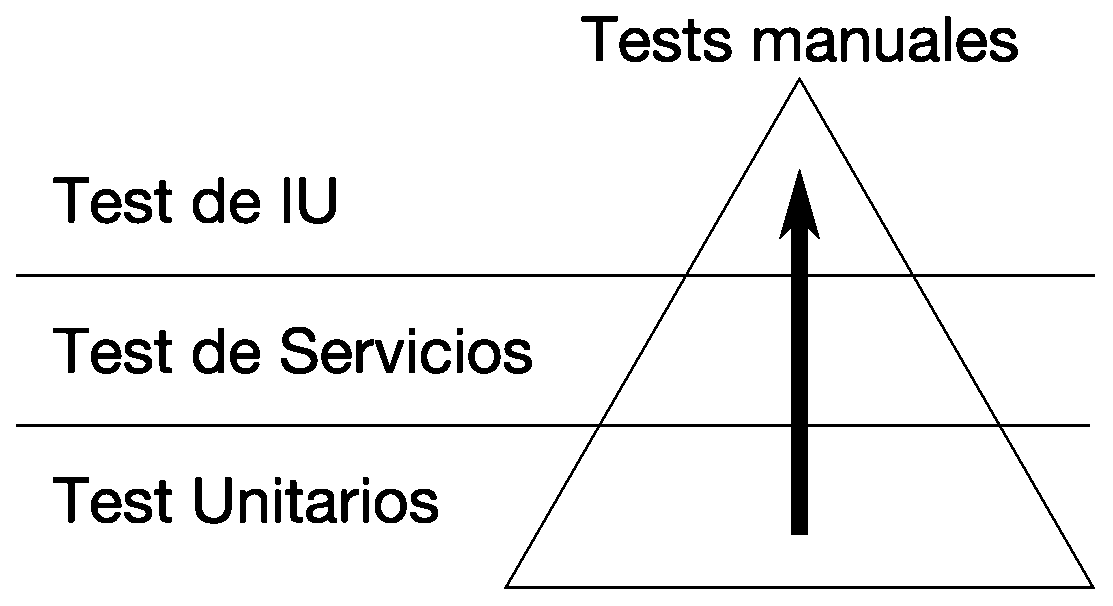
\includegraphics[width=0.5\textwidth]{graphics/pyramid.eps}
\caption{Pirámide de testing. Elaboración propia.}
\label{piramide}
\end{figure}

Las pruebas unitarias son rápidas y fiables, las pruebas en la capa de servicios
permiten evaluar la lógica del negocio donde la interfaz de usuario no esta
involucrada, cuanto mas alto sea el nivel en la pirámide, mas lentas y frágiles
resultan las pruebas.

Finalmente aunque se debe realizar alguna automatización de las pruebas de
interfaz de usuario, estas pruebas son mas lentas, mas difíciles de mantener y
se llegan a fallar mas fácilmente.

\subsection{La capa de interfaz}
Cuando el foco de la evaluación es la interfaz de usuario, se requiere que la
mayoría del código y la lógica de negocio este completamente evaluados. El
enfoque ahora se centra en simplemente asegurarse de que la propia interfaz de
usuario este funcionando correctamente. Las pruebas de interfaz de usuario son
muy frágiles, estas pruebas necesitaran mantenerse en cualquier momento que
cambie la interfaz de usuario, y como hay muchos factores que entran en juego
cuando se ejecuta una prueba que emula clics en una pantalla, estas pruebas
pueden dar como resultado falsos negativos. Estas fallas en las pruebas no
pueden ser ignoradas, pero tampoco debe gastarse mas tiempo en solucionar los
problemas y mantener las pruebas de UI que en encontrar defectos de código
reales.

Con un solido diseño de pruebas, las pruebas sobre la interfaz de usuario
complementan muy bien el conjunto de pruebas de automatización.

\section{End-to-End Testing}
Las pruebas End-to-End es una metodología que se utiliza para probar si el flujo
de una aplicación se esta realizando según lo diseñado de principio a fin. El
propósito de llevar a cabo pruebas de extremo a extremo es identificar las
dependencias del sistema y garantizar que la información correcta se transmita
entre varios componentes del sistema. Toda la aplicación se prueba en un
escenario del mundo real, como la comunicación con la base de datos, la red, el
hardware, y otros.

La prueba generalmente se realiza en la capa UI y se usa para validar que el
proceso de negocio de extremo a extremo funciona en todos los sistemas como una
prueba "horizontal". A diferencia de las pruebas verticales que miden el
rendimiento hacia arriba y hacia abajo de las capas de la pila de tecnología,
las pruebas horizontales de extremo a extremo se utilizan para garantizar que
los procesos de negocio de misión crítica funcionen. Las pruebas se ejecutan en
la capa UI y miden si la prueba continúa o no al siguiente paso del proceso.

\subsection{Buenas prácticas para pruebas E2E}
Una prueba típica de E2E puede ser compleja, con múltiples pasos que requieren
mucho tiempo para realizarlos manualmente. Esta complejidad también puede hacer
que las pruebas E2E sean difíciles de automatizar y lentas de ejecutar, para
ayudar a administrar los costos de las pruebas automatizadas de E2E a la vez que
mantienen los beneficios, se recomienda seguir las siguientes practicas:

\begin{itemize}
    \item Mantener una perspectiva de usuario final.
    \item Limitar las pruebas de excepción.
    \item Aplicar análisis de riesgo.
    \item Ejecutar las pruebas en el orden correcto.
    \item Manejar apropiadamente el entorno de prueba.
    \item Separar la lógica de prueba de los elementos de interfaz de usuario.
    \item Manejar correctamente la espera de los elementos de interfaz de usuario.
    \item Escoger los dispositivos adecuados.
    \item Optimizar el proceso de configuración y desmontaje de la prueba.
\end{itemize}

\section{Frameworks de automatización}
La automatización generalmente se interpreta como el manejo automático de
procesos a través de algoritmos inteligentes que involucran poca o ninguna
intervención humana. En el caso del software, significa realizar varias pruebas
en aplicaciones de software utilizando herramientas de automatización que son
versiones con licencia o de código abierto. En términos técnicos, el framework
de automatización de pruebas es un conjunto personalizado de componentes
interactivos que facilitan la ejecución de las pruebas con rutinas y la
generación de reportes completos de los resultados de las pruebas.

Dependiendo de como se desee abordar la creación de un framework y los
requisitos de automatización del proyecto, se cuentan con diferentes
clasificaciones:

\begin{description}
    \item [Lineal:] Son aquellos que registran los pasos de prueba y luego
        reproducir la rutina automáticamente para realizar la prueba.
    \item [Basado en módulos:] Estos dividen la aplicación bajo pruebas (AUT) en
        varios módulos lógicos y poco acoplados. Para cada modulo se crea una
        rutina de prueba separada e independiente.
    \item [De arquitectura de biblioteca:] Estos requieren determinar los pasos
        comunes de las pruebas, agruparlos en funciones en una biblioteca de
        funciones y llamar estas funciones en las rutinas de prueba cuando sea
        necesario.
    \item [Basado en datos:] Se enfoca en separar la lógica de las rutinas de
        prueba y los datos utilizados. Con esto se puede hacer que las rutinas
        de prueba funcionen fácilmente para diferentes conjuntos de datos.
    \item [Orientado por palabras clave:] Se enfoca en separar la parte técnica
        o de codificación del caso de prueba y de los pasos de necesarios de la
        prueba, para facilitar a una persona no técnica a entender bien la
        automatización.
    \item [Híbrido:] Son la combinación de dos o mas marcos mencionados
        anteriormente, que intenta aprovechar los puntos fuertes y los
        beneficios de otros marcos para el entorno de prueba.
\end{description}


\chapter{Análisis del Software}

En este capítulo, se desarrollan los aspectos necesarios para la definición del
proceso de desarrollo del \emph{framework}, primeramente se hará referencia a
las cuestiones relacionadas con las fuentes de análisis utilizadas, y algunos
conceptos puntuales acerca del producto, y la descripción de las actividades
planificadas durante el proyecto.

Posteriormente se describirán los \emph{tours} realizados en el sistema como
parte del análisis de los elementos, los cálculos de valor limite realizados
sobre los formularios, para terminar condensando los casos de prueba
formulados.

\section{Entorno de proyecto}
Los primeros componentes que se describirán son los relacionados con el entorno
del proyecto, que son aquellos factores del contexto que incluyen recursos
necesarios, restricciones, y cualquier otro elemento del proyecto que debe ser
tomado en cuenta para la evaluación.

\subsection{Fuentes de Información}
Para evaluar los componentes definidos en el proyecto, se encontraron
y recurrirán a las siguientes fuentes de información respecto al producto:

\begin{description}
\item [Centro de Ayuda] \emph{Salesforce} ofrece un amplio conjunto de
documentación, información general, preguntas frecuentes, y contacto con el
servicio de asistencia técnica desde su sitio de ayuda
(\emph{https://help.salesforce.com/}).

Estos recursos serán útiles para conocer los reclamos de los usuarios, las
características criticas del producto, y las estrategias del fabricante hacia
sus clientes.

\item [Centro de Desarrollo] \emph{Salesforce} también posee un sitio web
específicamente para compartir recursos de desarrollo sobre la plataforma
(\emph{https://developer.salesforce.com/}).

Este sitio se podrá aprovechar para consultar las referencias a las \emph{API}
del servicio, conocer las posibilidades que proveen los componentes y como
pueden aprovecharse desde la perspectiva del desarrollador.

\item [Recursos para administradores] Sitio web enfocado a ofrecer experiencias,
vídeos, herramientas, y un sin fin de recursos orientados a usuarios con un rol
administrativo de recursos sobre la plataforma
(\emph{https://admin.salesforce.com/resources}).

Este sitio será útil para entender las diferencias existentes entre la
funcionalidad provista a un usuario normal y a otro administrador, además de
conocer los permisos y roles de usuario en profundo.

\item [Comunidad \emph{Trailblazer}] Sitio web enfocado a conectar a miembros de
la comunidad \emph{Salesforce}, para compartir experiencias, aprender, y proveer
de nuevas ideas sobre la utilización del servicio
(\emph{https://success.salesforce.com/}).

Este sitio también sirve como fuente de reclamos de los usuarios,
funcionalidades criticas, y errores comunes encontrados en el servicio.

\end{description}

\subsection{\emph{Salesforce}}
\emph{Salesforce} cuenta con múltiples ediciones que comparten una apariencia,
pero varían según la funcionalidad y los costos del servicio. Según la
documentación del fabricante algunos clientes comienzan con una edición básica y
actualizan a una edición más rica en características a medida que evolucionan
los requisitos empresariales.

En el \emph{cuadro \ref{ediciones}} se describen las ediciones disponibles con
las que cuenta el servicio actualmente, cabe comentar que la evaluación se
realizará sobre la versión \emph{Developer} debido a que está es la que requiere
para su utilización, la menor cantidad de restricciones de parte del fabricante.

\begin{table}
\centering
\begin{tabular}{|l|p{12.0cm}|}
\hline
\footnotesize{\textbf{Edición}} & \footnotesize{\textbf{Descripción}} \\
\hline
\footnotesize{\emph{Essentials}} & \footnotesize{Diseñado para pequeños negocios
para empezar a trabajar con un sistema de \emph{CRM} de forma rápida. Incluye
presentaciones interactivas y un asistente de configuración para comenzar, una
interfaz de usuario fácil de utilizar y herramientas de administración para
personalizar su implementación conforme crece.} \\
\footnotesize{\emph{Professional}} & \footnotesize{Diseñado para negocios que
requieren la funcionalidad completa de \emph{CRM}. Incluye herramientas de
personalización, integración y administración directas y fáciles de usar para
facilitar cualquier implementación de pequeño y mediano tamaño.} \\
\footnotesize{\emph{Enterprise}} & \footnotesize{Cumple las necesidades
comerciales grandes y complejas. Proporciona herramientas avanzadas de
personalización y administración, además de todas las funcionalidades
disponibles en \emph{Professional Edition}, que pueden admitir implementaciones
a gran escala. \emph{Enterprise Edition} también incluye acceso a las \emph{API}
de \emph{Salesforce} para que pueda integrar fácilmente sistemas de gestión
interna.} \\
\footnotesize{\emph{Unlimited}} & \footnotesize{Proporciona nuevos niveles de
flexibilidad de plataforma para gestionar y compartir toda su información según
demanda. Incluye todas las funcionalidades de \emph{Enterprise Edition} además
de \emph{Premier Support}, acceso móvil completo, aplicaciones personalizadas
sin límite, límites de almacenamiento ampliados y otras funciones.} \\
\footnotesize{\emph{Developer}} & \footnotesize{Proporciona acceso a las
\emph{API} y la plataforma \emph{Lightning}. Permite a los desarrolladores
ampliar \emph{Salesforce}, integrarlo con otras aplicaciones y desarrollar
nuevas herramientas y aplicaciones. \emph{Developer Edition} ofrece además
acceso a muchas de las funciones disponibles en \emph{Enterprise Edition.}} \\
\hline
\end{tabular}
\caption{Ediciones actualmente disponibles de \emph{Sales Cloud}.}
\label{ediciones}
\source{https://help.salesforce.com/articleView?id=overview\_edition.htm}
\end{table}

Otra característica actual de \emph{Salesforce} es que cuenta con dos interfaces
web diferentes: la antigua conocida como: \emph{Salesforce Classic}, y la nueva
incluida desde 2015 denominada: \emph{Salesforce Lightning}; que tiene como
objetivo principal la unificación del comportamiento y la apariencia a través de
todo el servicio sea cual sea el dispositivo que el cliente
utilice \parencite{McCarthy}.

Se evaluarán las funcionalidades de los módulos sobre el navegador cuya
participación en el mercado es la mayor, en este caso: \emph{Google Chrome}
como puede verse en la \emph{figura \ref{software}}, priorizando las pruebas
sobre resoluciones de pantalla no menores a 1024 píxeles por 768 píxeles.

\begin{figure}
\centering
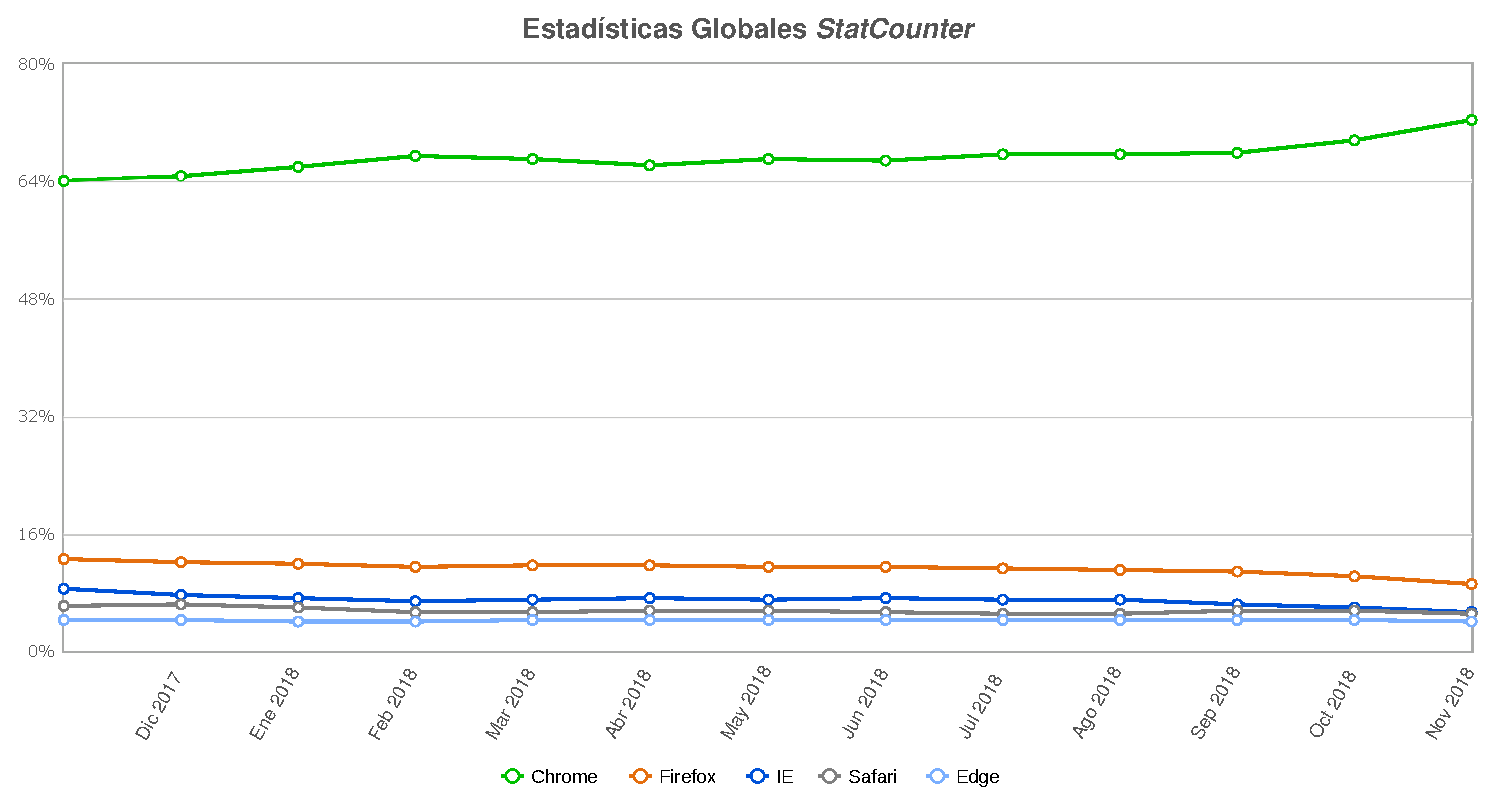
\includegraphics[width=1.0\textwidth]{graphics/compatibilidad.eps}
\caption{Participación de mercado de los navegadores hasta Noviembre del 2018.}
\label{software}
\source{http://gs.statcounter.com/browser-market-share/desktop/worldwide}
\end{figure}

Adicionalmente al uso del navegador \emph{Google Chrome} serán necesarios
otros navegadores para realizar la evaluación de compatibilidad sobre
vistas especificas del sistema, para este fin se consultó la información
disponible en la pagina de soporte provista por el fabricante, la cual como
puede verse en el \emph{cuadro \ref{soporte_navegadores}}, revela que se
soportan cinco navegadores diferentes bajo condiciones de limitación descritas
por el fabricante.

\begin{table}
\centering
\begin{tabular}{|p{6.0cm}|p{2.5cm}|p{1.4cm}|p{1.3cm}|p{1.3cm}|p{1.0cm}|}
\hline
& \footnotesize{\textbf{\emph{Microsoft Internet Explorer}}}
& \footnotesize{\textbf{\emph{Microsoft Edge}}}
& \footnotesize{\textbf{\emph{Google Chrome}}}
& \footnotesize{\textbf{\emph{Mozilla Firefox}}}
& \footnotesize{\textbf{\emph{Apple Safari}}} \\
\hline
\footnotesize{\emph{Lightning Experience}}
& \footnotesize{IE11 (EOL Diciembre 31, 2020)}
& \footnotesize{Ultima versión}
& \footnotesize{Ultima versión}
& \footnotesize{Ultima versión}
& \footnotesize{11.x+} \\
\footnotesize{\emph{Lightning Communities}}
& \footnotesize{IE11 (EOL Diciembre 31, 2020)}
& \footnotesize{Ultima versión}
& \footnotesize{Ultima versión}
& \footnotesize{Ultima versión}
& \footnotesize{11.x+} \\
\footnotesize{¿Consideraciones especiales de configuración?}
& \footnotesize{No}
& \footnotesize{No}
& \footnotesize{No}
& \footnotesize{No}
& \footnotesize{No} \\
\footnotesize{Limitaciones conocidas}
& \footnotesize{Sí}
& \footnotesize{Si}
& \footnotesize{No}
& \footnotesize{Si}
& \footnotesize{Si} \\
\hline
\end{tabular}
\caption{Lista de compatibilidad provista por \emph{Salesforce}.}
\label{soporte_navegadores}
\source{https://help.salesforce.com/articleView?id=getstart\_browsers\_sfx.htm}
\end{table}

\section{Planificación de actividades}
Para conseguir los objetivos planteados por el proyecto se realizarán las
actividades detalladas en el \emph{cuadro \ref{planificacion}} en la página
\pageref{planificacion}. Este cuadro detalla las actividades agrupadas por el
objetivo especifico y detallando también el resultado esperado de estas.

\begin{sidewaystable}
\renewcommand{\arraystretch}{1}
\linespread{1.25}
\centering
\small
\begin{tabular}{|l|l|p{6.5cm}|l|}
\hline
Objetivo General & Objetivos Específicos & Actividades & Resultados \\
\hline
\multirow{10}{4.0cm}{Implementar un \emph{framework} para la automatización de
las pruebas de interfaz de usuario en el módulo de Productos y Listas de Precios
en \emph{Salesforce}, para garantizar un procedimiento continuo de evaluación y
minimizar la cantidad de errores que contiene el software.} &
\multirow{3}{4.0cm}{Formular los casos de prueba necesarios que los módulos de
gestión de productos y listas de precios requieran para cubrir los atributos de
calidad requeridos.} &
Recolección de la información y exploración de los módulos específicos. &
\multirow{3}{4.0cm}{Casos de prueba para los módulos de Productos y Listas de
Precios.} \\
\cline{3-3}
& & Análisis y diseño de los tipos de evaluación requeridos para los módulos
específicos. & \\
\cline{3-3}
& & Formulación los casos de prueba necesarios para los módulos
específicos. & \\
\cline{2-4}
& \multirow{3}{4.0cm}{Diseñar e implementar los modelos y bibliotecas de
funciones que conforman un \emph{framework} de automatización.} &
Análisis y modelamiento de los componentes del \emph{framework}. &
\multirow{3}{4.0cm}{\emph{Framework} de automatización con los componentes
necesarios para la implementación de los casos de prueba.} \\
\cline{3-3}
& & Estructuración de los entornos de prueba y configuración de los servicios
disponibles. & \\
\cline{3-3}
& & Implementación de los componentes del \emph{framework}. & \\
\cline{2-4}
& \multirow{4}{4.0cm}{Automatizar los casos de prueba de las funciones que
componen la interfaz de usuario del módulo de gestión de productos y listas de
precios.} &
Implementación de los casos de prueba formulados. &
\multirow{4}{4.0cm}{Rutinas de automatización de los casos de prueba de los
módulos de Productos y Listas de Precios.} \\
\cline{3-3}
& & Implementación de pre condiciones y post condiciones en la ejecución de los
casos de prueba. & \\
\cline{3-3}
& & Ejecución de los casos de prueba automatizados. & \\
\cline{3-3}
& & Generación del reporte de resultados y reporte de errores. & \\
\hline
\end{tabular}
\caption{Planificación de actividades del proyecto.}
\label{planificacion}
\source{Elaboración propia.}
\end{sidewaystable}

\section{Elementos del producto}
Dentro del alcance de la evaluación se encuentran los componentes de productos
y listas de precios, las funcionalidades que comprenden estos se detallan en
esta sección, desde múltiples perspectivas de análisis.

Como se mencionó anteriormente, se consideró la interfaz
\emph{Lightning Experience}, como único objetivo de la evaluación. La versión
\emph{Lightning Experience} esta disponible para las siguientes ediciones del
producto: \emph{Essentials}, \emph{Group}, \emph{Professional},
\emph{Enterprise}, \emph{Performance}, \emph{Unlimited}, y \emph{Developer}.

\subsection{Productos}
El Producto para el software a evaluar, representa uno de los componentes
fundamentales y claves para el éxito, por ende es importante evaluarlo
desde múltiples facetas; la primera de estas es la funcionalidad provista por
las interfaces de este módulo. En la \emph{figura \ref{productos}} pueden verse
estas funcionalidades, clasificadas desde la perspectiva de la interfaz de
usuario.

Entre las funcionalidades que pueden apreciarse están las operaciones comunes
de creación, búsqueda, visualización, modificación, y eliminación de productos,
se omitieron las funcionalidades de controles de vista de lista, para que
todo este componente pueda ser tratado de manera separada. También pueden
observarse funciones relacionadas a registrar precios estándar y precios para
una lista de precios determinada.

En la \emph{figura \ref{productos_vistas}}, se aprecian las diferentes vistas
que comprenden el módulo, se resaltó con color amarillo aquellas vistas que son
de tipo formulario, mientras que se resaltó con color verde aquellas que son de
tipo confirmación de acción.

Además de las funcionalidades y vistas antes mencionadas, también se analizó el
comportamiento de los formularios que provee el módulo, como puede verse en la
\emph{figura \ref{productos_formularios}}.

\begin{figure}
\centering
\begin{tikzpicture}[
    grow via three points={one child at (0.5,-0.7) and
    two children at (0.5,-0.7) and (0.5,-1.4)},
    edge from parent path={(\tikzparentnode.south) |- (\tikzchildnode.west)}]
    \node {Productos}
        child { node {Nuevo}}
        child { node {Buscar: Producto}}
        child { node {Controles de Vista de Lista}
            child { node {\ldots}}
        }
        child [missing] {}
        child { node {Mostrar como}}
        child { node {Actualizar}}
        child { node {Filtrar por: Vista de Lista}}
        child { node {Modificar Lista}}
        child { node {Lista de Productos}
            child { node {Ver: Producto}
                child { node {Modificar}}
                child { node {Eliminar}}
                child { node {Duplicar}}
                child { node {Relacionado}
                    child { node {Agregar precio estándar}}
                    child { node {Agregar a lista de precios}}
                    child { node {Ver: Lista de precios}}
                    child { node {Modificar: Lista de precios}}
                    child { node {Eliminar: Lista de precios}}
                    child { node {Ver todos}
                        child { node {Actualizar}}
                    }
                }
                child [missing] {}
                child [missing] {}
                child [missing] {}
                child [missing] {}
                child [missing] {}
                child [missing] {}
                child [missing] {}
                child { node {Detalles}}
            }
            child [missing] {}
            child [missing] {}
            child [missing] {}
            child [missing] {}
            child [missing] {}
            child [missing] {}
            child [missing] {}
            child [missing] {}
            child [missing] {}
            child [missing] {}
            child [missing] {}
            child [missing] {}
            child { node {Modificar: Producto}}
            child { node {Eliminar: Producto}}
        };
\end{tikzpicture}
\caption{Funciones que componen el módulo de gestión de productos.}
\label{productos}
\source{Elaboración propia.}
\end{figure}

\begin{figure}
\centering
\begin{tikzpicture}[
    grow via three points={one child at (0.5,-0.7) and
    two children at (0.5,-0.7) and (0.5,-1.4)},
    edge from parent path={(\tikzparentnode.south) |- (\tikzchildnode.west)}]
    \node {Productos}
        child { node {Mostrar como}
            child { node {Tabla}}
            child { node {Kanban}}
        }
        child [missing] {}
        child [missing] {}
        child { node [form] {Crear Producto}}
        child { node {Filtros}}
        child { node {Producto}
            child { node [form] {Modificar: Producto}}
            child { node [confirm] {Eliminar: Producto}}
            child { node [form] {Crear Producto}}
            child { node {Detalles}}
            child { node {Relacionado}
                child { node [form] {Crear Entrada del catalogo de precios}}
                child { node [form] {Agregar a lista de precios}}
                child { node {Listas de precios}
                    child { node [form] {Modificar Entrada del catalogo de precios}}
                    child { node [confirm] {Eliminar entrada del catalogo de precios}}
                }
            }
        }
        child [missing] {}
        child [missing] {}
        child [missing] {}
        child [missing] {}
        child [missing] {}
        child [missing] {}
        child [missing] {}
        child [missing] {}
        child [missing] {}
        child [missing] {}
        child { node [form] {Modificar: Producto}}
        child { node [confirm] {Eliminar: Producto}};
\end{tikzpicture}
\caption{Vistas que componen el módulo de gestión de productos.}
\label{productos_vistas}
\source{Elaboración propia.}
\end{figure}

\begin{figure}
\centering
\begin{tikzpicture}[
    grow via three points={one child at (0.5,-0.7) and
    two children at (0.5,-0.7) and (0.5,-1.4)},
    edge from parent path={(\tikzparentnode.south) |- (\tikzchildnode.west)}]
    \node {Productos}
        child { node {Crear producto}
            child { node {Nombre del producto (*)}}
            child { node {Activo}}
            child { node {Código de producto}}
            child { node {Familia de productos}}
            child { node {Descripción del producto}}
        }
        child [missing] {}
        child [missing] {}
        child [missing] {}
        child [missing] {}
        child [missing] {}
        child { node {Crear entrada del catálogo de precios}
            child { node {Producto (*)}}
            child { node {Activo}}
            child { node {Lista de precios (*)}}
            child { node {Precio de la lista (*)}}
            child { node {Utilizar precio estándar}}
        }
        child [missing] {}
        child [missing] {}
        child [missing] {}
        child [missing] {}
        child [missing] {}
        child { node {Agregar a lista de precios}
            child { node {Lista de precios (*)}}
            child { node {Divisa (*)}}
        }
        child [missing] {}
        child [missing] {}
        child { node {Modificar entrada del catálogo de precios}
            child { node {Activo}}
            child { node {Precio de la lista (*)}}
            child { node {Utilizar precio estándar}}
        };
\end{tikzpicture}
\caption{Formularios que componen el módulo de gestión de productos.}
\label{productos_formularios}
\source{Elaboración propia.}
\end{figure}

\subsection{Listas de Precios}
Las Listas de Precios, tienen como objetivo, hacer que un mismo producto pueda
tener múltiples precios, dependiendo de como la organización cliente maneje sus
canales de distribución y producción. Al igual que en el módulo de productos, en
la \emph{figura \ref{listas_de_precios}} pueden verse las funcionalidades
clasificadas desde la perspectiva de la interfaz de usuario, también se omitió
la sección de los controles de vista de lista.

Las funciones de Listas de Precios son muy similares a aquellas vistas en el
módulo de productos, analizado anteriormente.

En la \emph{figura \ref{listas_de_precios_vistas}}, se detallan aquellas vistas
presentes en este módulo, de la misma manera se ha destacado con amarillo a
aquellas vistas que son formularios, mientras que en verde se presentan a
aquellas que representan diálogos de confirmación.

También de las funcionalidades y vistas antes mencionadas, se analizó el
comportamiento de los formularios que provee este módulo, como puede verse en la
\emph{figura \ref{listas_de_precios_formularios}}.

\begin{figure}
\centering
\begin{tikzpicture}[
    grow via three points={one child at (0.5,-0.7) and
    two children at (0.5,-0.7) and (0.5,-1.4)},
    edge from parent path={(\tikzparentnode.south) |- (\tikzchildnode.west)}]
    \node {Listas de Precios}
        child { node {Nuevo}}
        child { node {Buscar: Lista de precios}}
        child { node {Controles de Vista de Lista}
            child { node {\ldots}}
        }
        child [missing] {}
        child { node {Mostrar como}}
        child { node {Actualizar}}
        child { node {Filtrar por: Vista de Lista}}
        child { node {Modificar Lista}}
        child { node {Lista de Listas de Precios}
            child { node {Ver: Lista de precios}
                child { node {Modificar}}
                child { node {Eliminar}}
                child { node {Duplicar}}
                child { node {Relacionado}
                    child { node {Agregar productos}}
                    child { node {Ver: Producto}}
                    child { node {Modificar: Producto}}
                    child { node {Eliminar: Producto}}
                    child { node {Ver todos}
                        child { node {Actualizar}}
                    }
                    child [missing] {}
                    child { node {Historial de lista de precios (Ver todos)}
                        child { node {Actualizar}}
                    }
                }
                child [missing] {}
                child [missing] {}
                child [missing] {}
                child [missing] {}
                child [missing] {}
                child [missing] {}
                child [missing] {}
                child [missing] {}
                child { node {Detalles}}
            }
            child [missing] {}
            child [missing] {}
            child [missing] {}
            child [missing] {}
            child [missing] {}
            child [missing] {}
            child [missing] {}
            child [missing] {}
            child [missing] {}
            child [missing] {}
            child [missing] {}
            child [missing] {}
            child [missing] {}
            child { node {Modificar: Lista de Precios}}
            child { node {Eliminar: Lista de Precios}}
        };
\end{tikzpicture}
\caption{Funciones que componen el módulo de gestión de listas de precios.}
\label{listas_de_precios}
\source{Elaboración propia.}
\end{figure}

\begin{figure}
\centering
\begin{tikzpicture}[
    grow via three points={one child at (0.5,-0.7) and
    two children at (0.5,-0.7) and (0.5,-1.4)},
    edge from parent path={(\tikzparentnode.south) |- (\tikzchildnode.west)}]
    \node {Listas de Precios}
        child { node {Mostrar como}
            child { node {Tabla}}
            child { node {Kanban}}
        }
        child [missing] {}
        child [missing] {}
        child { node [form] {Crear Lista de precios}}
        child { node {Filtros}}
        child { node {Lista de precios}
            child { node [form] {Modificar: Lista de Precios}}
            child { node [form] {Crear Lista de precios}}
            child { node [confirm] {Eliminar: Lista de precios}}
            child { node {Detalles}}
            child { node {Relacionado}
                child { node [form] {Agregar productos}
                    child { node [form] {Modificar Entrada del catalogo de precios}}
                }
                child [missing] {}
                child { node {Productos}
                    child { node [form] {Modificar Entrada del catalogo de precios}}
                    child { node [confirm] {Eliminar Entrada del catalogo de precios}}
                }
                child [missing] {}
                child [missing] {}
                child { node {Historial de lista de precios}}
            }
        }
        child [missing] {}
        child [missing] {}
        child [missing] {}
        child [missing] {}
        child [missing] {}
        child [missing] {}
        child [missing] {}
        child [missing] {}
        child [missing] {}
        child [missing] {}
        child [missing] {}
        child { node [form] {Modificar: Lista de Precio}}
        child { node [confirm] {Eliminar: Lista de Precio}};
\end{tikzpicture}
\caption{Vistas que componen el módulo de gestión de listas de precios.}
\label{listas_de_precios_vistas}
\source{Elaboración propia.}
\end{figure}

\begin{figure}
\centering
\begin{tikzpicture}[
    grow via three points={one child at (0.5,-0.7) and
    two children at (0.5,-0.7) and (0.5,-1.4)},
    edge from parent path={(\tikzparentnode.south) |- (\tikzchildnode.west)}]
    \node {Listas de Precios}
        child { node {Crear lista de precios}
            child { node {Nombre de la lista de precios (*)}}
            child { node {Activo}}
            child { node {Descripción}}
            child { node {Es lista de precios estándar}}
        }
        child [missing] {}
        child [missing] {}
        child [missing] {}
        child [missing] {}
        child { node {Agregar productos}
            child { node {Buscar entrada de catálogos de precios}
                child { node {Modificar Entrada de catálogos de precios}}
            }
        };
\end{tikzpicture}
\caption{Formularios que componen el módulo de gestión de listas de precios.}
\label{listas_de_precios_formularios}
\source{Elaboración propia.}
\end{figure}

\subsection{Controles de Vista de Lista}
Los Controles de Vista de Lista son funcionalidades equivalentes entre los 
dos componentes que están siendo evaluados, por lo que se ha decidido realizar
un análisis separado de estos. En la \emph{figura \ref{vista_de_lista}} puede
verse las funciones omitidas en los diagramas anteriores relativas a los
controles de vista.

En la \emph{figura \ref{vista_de_lista_vistas}}, se detallan aquellas vistas
provistas por este componente, de la misma manera que en los dos módulos
anteriormente citados, aquí también se han destacado con amarillo a
aquellas vistas que son formularios, mientras que en verde se presentan a
aquellas que representan diálogos de confirmación.

También de las funcionalidades y vistas antes mencionadas, se analizó el
comportamiento de los formularios que provee este módulo, como puede verse en la
\emph{figura \ref{vista_de_lista_formularios}}.

\begin{figure}
\centering
\begin{tikzpicture}[
    grow via three points={one child at (0.5,-0.7) and
    two children at (0.5,-0.7) and (0.5,-1.4)},
    edge from parent path={(\tikzparentnode.south) |- (\tikzchildnode.west)}]
    \node {Controles de Vista de Lista}
        child { node {Nuevo}}
        child { node {Duplicar}}
        child { node {Cambiar nombre}}
        child { node {Configuración de colaboración}
            child { node {Modificar}}
        }
        child [missing] {}
        child { node {Modificar filtros de lista}
            child { node {Ver/Modificar: Filtro}}
            child { node {Eliminar: Filtro}}
            child { node {Agregar Filtro}}
            child { node {Eliminar todos}}
            child { node {Agregar lógica de filtro}}
        }
        child [missing] {}
        child [missing] {}
        child [missing] {}
        child [missing] {}
        child [missing] {}
        child { node {Seleccionar los campos que se visualizaran}}
        child { node {Eliminar}}
        child { node {Restablecer anchuras de columna}}
        child { node {Configuración de Kanban}};
\end{tikzpicture}
\caption{Funciones que componen el módulo de gestión de vistas de lista.}
\label{vista_de_lista}
\source{Elaboración propia.}
\end{figure}

\begin{figure}[H]
\centering
\begin{tikzpicture}[
    grow via three points={one child at (0.5,-0.7) and
    two children at (0.5,-0.7) and (0.5,-1.4)},
    edge from parent path={(\tikzparentnode.south) |- (\tikzchildnode.west)}]
    \node {Vista de Lista}
        child { node [form] {Nueva vista de lista}}
        child { node [form] {Duplicar vista de lista}}
        child { node [form] {Cambiar nombre}}
        child { node [form] {Configuración de colaboración}}
        child { node [form] {Seleccionar los campos que se visualizaran}}
        child { node [confirm] {Eliminar}}
        child { node [form] {Configuración de Kanban}};
\end{tikzpicture}
\caption{Vistas que componen el módulo de gestión de listas de precios.}
\label{vista_de_lista_vistas}
\source{Elaboración propia.}
\end{figure}

\begin{figure}
\centering
\begin{tikzpicture}[
    grow via three points={one child at (0.5,-0.7) and
    two children at (0.5,-0.7) and (0.5,-1.4)},
    edge from parent path={(\tikzparentnode.south) |- (\tikzchildnode.west)}]
    \node {Vista de lista}
        child { node {Nueva vista de lista}
            child { node {Nombre de la lista (*)}}
            child { node {List API Name (*)}}
            child { node {¿Quien ve esta vista de lista?}
                child { node {Solo yo puedo ver esta vista de lista}}
                child { node {Todos los usuarios pueden ver esta vista de lista}}
                child { node {Compartir vista de lista con grupos de usuarios}}
            }
        }
        child [missing] {}
        child [missing] {}
        child [missing] {}
        child [missing] {}
        child [missing] {}
        child [missing] {}
        child { node {Cambiar nombre}
            child { node {Nombre de lista (*)}}
        }
        child [missing] {}
        child { node {Configuración de colaboración}
            child { node {¿Quien ve esta vista de lista?}
                child { node {Solo yo puedo ver esta vista de lista}}
                child { node {Todos los usuarios pueden ver esta vista de lista}}
                child { node {Compartir vista de lista con grupos de usuarios}}
            }
        }
        child [missing] {}
        child [missing] {}
        child [missing] {}
        child [missing] {}
        child { node {Agregar filtro}
            child { node {Campo}}
            child { node {Operador}}
            child { node {Valor}}
        }
        child [missing] {}
        child [missing] {}
        child [missing] {}
        child { node {Agregar lógica de filtro}
            child { node {Lógica de filtro}}
        }
        child [missing] {}
        child { node {Seleccionar los campos que se visualizaran}
            child { node {Campos disponibles}}
            child { node {Campos visibles (*)}}
        }
        child [missing] {}
        child [missing] {}
        child { node {Configuración de Kanban}
            child { node {Resumir por)}}
            child { node {Agrupar por (*)}}
        };
\end{tikzpicture}
\caption{Formularios que componen el módulo de gestión de vistas de listas.}
\label{vista_de_lista_formularios}
\source{Elaboración propia.}
\end{figure}

\section{Análisis de valor limite}
Para el análisis de los formularios se crearon las respectivas tablas producidas
a partir del análisis de sus valores limite, las cuales son descritas a
continuación:

\begin{itemize}
    \item Crear Producto, que puede verse en el \emph{cuadro \ref{myers_01}}.
    \item Crear Entrada del catalogo de precios, que puede verse en el
        \emph{cuadro \ref{myers_02}}.
    \item Agregar a lista de precios, que puede verse en el
        \emph{cuadro \ref{myers_03}}.
    \item Modificar Entrada del catalogo de precios, que puede verse en el
        \emph{cuadro \ref{myers_04}}.
    \item Crear Lista de precios, que puede verse en el
        \emph{cuadro \ref{myers_05}}.
    \item Agregar productos, que puede verse en el \emph{cuadro \ref{myers_06}}.
    \item Nueva vista de lista, que puede verse en el
        \emph{cuadro \ref{myers_07}}.
    \item Cambiar nombre, que puede verse en el \emph{cuadro \ref{myers_08}}.
    \item Configuración de colaboración, que puede verse en el
        \emph{cuadro \ref{myers_09}}.
\end{itemize}

\begin{table}
\centering
\begin{tabular}{|p{6.0cm}|l|l|l|}
\hline
\footnotesize{\textbf{Variable}} & \footnotesize{\textbf{Casos Posibles}} & \footnotesize{\textbf{Casos Inválidos}} & \footnotesize{\textbf{Limites}} \\
\hline
\footnotesize{Nombre del producto} & \footnotesize{[1-255] caracteres} & & \footnotesize{0} \\
& & \footnotesize{0} & \footnotesize{1} \\
& & \footnotesize{$>$255} & \footnotesize{255} \\
& & & \footnotesize{256} \\
\hline
\footnotesize{Activo} & \footnotesize{\{verdadero,falso\}} & & \\
\hline
\footnotesize{Código de producto} & \footnotesize{[0-255] caracteres} & & \footnotesize{0} \\
& & \footnotesize{$>$255} & \footnotesize{255} \\
& & & \footnotesize{256} \\
\hline
\footnotesize{Familia de productos} & \footnotesize{ninguno,[lista de valores]} & & \\
\hline
\footnotesize{Programación de cantidades activada} & \footnotesize{\{verdadero,falso\}} & & \\
\hline
\footnotesize{Programación de ingresos activada} & \footnotesize{\{verdadero,falso\}} & & \\
\hline
\footnotesize{Descripción del producto} & \footnotesize{[0,4000] caracteres} & & \footnotesize{0} \\
& & \footnotesize{$>$4000} & \footnotesize{4000} \\
& & & \footnotesize{4001} \\
\hline
\end{tabular}
\caption{Análisis de valor limite para el formulario «Crear Producto»}
\label{myers_01}
\source{Elaboración propia.}
\end{table}

\begin{table}
\centering
\begin{tabular}{|p{3.0cm}|p{4.0cm}|p{4.0cm}|l|}
\hline
\footnotesize{\textbf{Variable}} & \footnotesize{\textbf{Casos Posibles}} & \footnotesize{\textbf{Casos Inválidos}} & \footnotesize{\textbf{Limites}} \\
\hline
\footnotesize{Producto} & \footnotesize{[lista de valores]} & & \\
\hline
\footnotesize{Activo}  & \footnotesize{\{verdadero,falso\}} & & \\
\hline
\footnotesize{Lista de precios} & \footnotesize{[lista de valores]} & & \\
\hline
\footnotesize{Precio de la lista} & \footnotesize{[} & \footnotesize{$<$-9.007.199.254.740.991} & \footnotesize{-9.007.199.254.740.992} \\
& \footnotesize{-9.007.199.254.740.991} & & \footnotesize{-9.007.199.254.740.991} \\
& \footnotesize{9.007.199.254.740.991} & & \footnotesize{9.007.199.254.740.991} \\
& \footnotesize{]} & \footnotesize{$>$9.007.199.254.740.991} & \footnotesize{9.007.199.254.740.992} \\
& \footnotesize{3 decimales} & & \footnotesize{0,999} \\
& & \footnotesize{4 decimales} & \footnotesize{0,9999} \\
\hline
\footnotesize{Utilizar Precio estándar} & \footnotesize{\{verdadero,falso\}} & & \\
\hline
\end{tabular}
\caption{Análisis de valor limite para el formulario «Crear Entrada del catalogo de precios»}
\label{myers_02}
\source{Elaboración propia.}
\end{table}

\begin{table}
\centering
\begin{tabular}{|p{6.0cm}|l|l|l|}
\hline
\footnotesize{\textbf{Variable}} & \footnotesize{\textbf{Casos Posibles}} & \footnotesize{\textbf{Casos Inválidos}} & \footnotesize{\textbf{Limites}} \\
\hline
\footnotesize{Lista de precios} & \footnotesize{ninguno,[lista de valores]} & & \\
\hline
\footnotesize{Divisa} & \footnotesize{ninguno,[lista de valores]} & & \\
\hline
\end{tabular}
\caption{Análisis de valor limite para el formulario «Agregar a lista de precios»}
\label{myers_03}
\source{Elaboración propia.}
\end{table}

\begin{table}
\centering
\begin{tabular}{|p{3.0cm}|p{4.0cm}|p{4.0cm}|l|}
\hline
\footnotesize{\textbf{Variable}} & \footnotesize{\textbf{Casos Posibles}} & \footnotesize{\textbf{Casos Inválidos}} & \footnotesize{\textbf{Limites}} \\
\hline
\footnotesize{Activo} & \footnotesize{\{verdadero,falso\}} & & \\
\hline
\footnotesize{Precio de la lista} & \footnotesize{[} & \footnotesize{$<$-9.007.199.254.740.991} & \footnotesize{-9.007.199.254.740.992} \\
& \footnotesize{-9.007.199.254.740.991} & & \footnotesize{-9.007.199.254.740.991} \\
& \footnotesize{9.007.199.254.740.991} & & \footnotesize{9.007.199.254.740.991} \\
& \footnotesize{]} & \footnotesize{$>$9.007.199.254.740.991} & \footnotesize{9.007.199.254.740.992} \\
& \footnotesize{3 decimales} & & \footnotesize{0,999} \\
& & \footnotesize{4 decimales} & \footnotesize{0,9999} \\
\hline
\footnotesize{Utilizar precio estándar} & \footnotesize{\{verdadero,falso\}} & & \\
\hline
\end{tabular}
\caption{Análisis de valor limite para el formulario «Modificar Entrada del catalogo de precios»}
\label{myers_04}
\source{Elaboración propia.}
\end{table}

\begin{table}
\centering
\begin{tabular}{|p{6.0cm}|l|l|l|}
\hline
\footnotesize{\textbf{Variable}} & \footnotesize{\textbf{Casos Posibles}} & \footnotesize{\textbf{Casos Inválidos}} & \footnotesize{\textbf{Limites}} \\
\hline
\footnotesize{Nombre de la lista de precios} & \footnotesize{[1-255] caracteres} & & \footnotesize{0} \\
& & \footnotesize{0} & \footnotesize{1} \\
& & \footnotesize{$>$255} & \footnotesize{255} \\
& & & \footnotesize{256} \\
\hline
\footnotesize{Activo} & \footnotesize{\{verdadero,falso\}} & & \\
\hline
\footnotesize{Descripción del producto} & \footnotesize{[0,255] caracteres} & & \footnotesize{0} \\
& & \footnotesize{$>$255} & \footnotesize{255} \\
& & & \footnotesize{256} \\
\hline
\footnotesize{Es lista de precios estándar} & \footnotesize{\{verdadero,falso\}} & & \\
\hline
\end{tabular}
\caption{Análisis de valor limite para el formulario «Crear Lista de precios»}
\label{myers_05}
\source{Elaboración propia.}
\end{table}

\begin{table}
\centering
\begin{tabular}{|p{3.0cm}|p{4.0cm}|p{4.0cm}|l|}
\hline
\footnotesize{\textbf{Variable}} & \footnotesize{\textbf{Casos Posibles}} & \footnotesize{\textbf{Casos Inválidos}} & \footnotesize{\textbf{Limites}} \\
\hline
\footnotesize{Buscar Entrada de catálogos de precios\ldots} & \footnotesize{[1-500] caracteres} & & \footnotesize{0} \\
& & & \footnotesize{1} \\
& & & \footnotesize{500} \\
& & & \footnotesize{501} \\
\hline
\multicolumn{4}{|l|}{\footnotesize{Modificar Entrada de catálogos de precios seleccionada}} \\
\hline
\footnotesize{Activo} & \footnotesize{\{verdadero,falso\}} & & \\
\hline
\footnotesize{Precio de la lista} & \footnotesize{[} & \footnotesize{$<$-9.007.199.254.740.991} & \footnotesize{-9.007.199.254.740.992} \\
& \footnotesize{-9.007.199.254.740.991} & & \footnotesize{-9.007.199.254.740.991} \\
& \footnotesize{9.007.199.254.740.991} & & \footnotesize{9.007.199.254.740.991} \\
& \footnotesize{]} & \footnotesize{$>$9.007.199.254.740.991} & \footnotesize{9.007.199.254.740.992} \\
& \footnotesize{3 decimales} & & \footnotesize{0,999} \\
& & \footnotesize{4 decimales} & \footnotesize{0,9999} \\
\hline
\footnotesize{Utilizar Precio estándar} & \footnotesize{\{verdadero,falso\}} & & \\
\hline
\end{tabular}
\caption{Análisis de valor limite para el formulario «Agregar productos»}
\label{myers_06}
\source{Elaboración propia.}
\end{table}

\begin{table}
\centering
\begin{tabular}{|p{3.0cm}|p{7.0cm}|p{3.0cm}|l|}
\hline
\footnotesize{\textbf{Variable}} & \footnotesize{\textbf{Casos Posibles}} & \footnotesize{\textbf{Casos Inválidos}} & \footnotesize{\textbf{Limites}} \\
\hline
\footnotesize{Nombre de lista} & \footnotesize{[1-40] caracteres} & & \footnotesize{0} \\
& & \footnotesize{0} & \footnotesize{1} \\
& & \footnotesize{$>$40} & \footnotesize{40} \\
& & & \footnotesize{41} \\
\hline
\footnotesize{List API Name} & \footnotesize{[1-80]} & & \footnotesize{0} \\
& & \footnotesize{0} & \footnotesize{1} \\
& & \footnotesize{$>$80} & \footnotesize{80} \\
& & & \footnotesize{81} \\
& \footnotesize{[a-zA-Z][a-zA-Z0-9\_][a-zA-Z0-9]} & & \\
& & \footnotesize{1xxxxx} & \footnotesize{1xxxxx} \\
& & \footnotesize{\_xxxxx} & \footnotesize{\_xxxxx} \\
& & \footnotesize{xxx\_\_xxx} & \footnotesize{xxx\_\_xxx} \\
& & \footnotesize{xxxxx\_} & \footnotesize{xxxxx\_} \\
\hline
\footnotesize{¿Quien ve esta lista?} & \footnotesize{Solo yo puedo ver esta vista de lista} & & \\
& \footnotesize{Todos los usuarios pueden ver esta vista de lista} & & \\
& \footnotesize{Compartir vista de lista con grupos de usuarios} & & \\
\hline
\end{tabular}
\caption{Análisis de valor limite para el formulario «Nueva vista de lista»}
\label{myers_07}
\source{Elaboración propia.}
\end{table}

\begin{table}
\centering
\begin{tabular}{|l|l|l|l|}
\hline
\footnotesize{\textbf{Variable}} & \footnotesize{\textbf{Casos Posibles}} & \footnotesize{\textbf{Casos Inválidos}} & \footnotesize{\textbf{Limites}} \\
\hline
\footnotesize{Nombre de lista} & \footnotesize{[1-40] caracteres} & & \footnotesize{0} \\
& & \footnotesize{0} & \footnotesize{1} \\
& & \footnotesize{$>$40} & \footnotesize{40} \\
& & & \footnotesize{41} \\
\hline
\end{tabular}
\caption{Análisis de valor limite para el formulario «Cambiar nombre»}
\label{myers_08}
\source{Elaboración propia.}
\end{table}

\begin{table}
\centering
\begin{tabular}{|l|l|l|l|}
\hline
\footnotesize{\textbf{Variable}} & \footnotesize{\textbf{Casos Posibles}} & \footnotesize{\textbf{Casos Inválidos}} & \footnotesize{\textbf{Limites}} \\
\hline
\footnotesize{¿Quien ve esta lista?} & \footnotesize{Solo yo puedo ver esta vista de lista} & & \\
& \footnotesize{Todos los usuarios pueden ver esta vista de lista} & & \\
& \footnotesize{Compartir vista de lista con grupos de usuarios} & & \\
\hline
\end{tabular}
\caption{Análisis de valor limite para el formulario «Configuración de colaboración»}
\label{myers_09}
\source{Elaboración propia.}
\end{table}

\section{Casos de prueba}
A partir del análisis realizado, se terminó formulando múltiples casos de
prueba, estos se encuentran descritos en el \emph{\textbf{apéndice
\ref{appendix_testscases}}} categorizados e individualizados según el área y
subarea al que pertenecen.

En la \emph{figura \ref{tc-tests}}, se puede ver la distribución de los casos de
prueba según el tipo de evaluación realizado, puede apreciarse que las pruebas
funcionales ocupan mas de la mitad de la totalidad de casos de prueba en el
proyecto, mientras que los casos de prueba negativos, y de aceptación, están más
próximos al 10\%.

En la \emph{figura \ref{tc-type}}, se puede ver la distribución de los casos de
prueba según el tipo de acción que se realiza en el sistema, es decir, si son
casos que afectan la interfaz de usuario, si mas bien son funciones de
validación, o si realizan alguna petición al servidor, sea esta de lectura o
escritura.

Puede apreciarse igualmente que la mayor parte de los casos de prueba están
orientados a evaluar el comportamiento de la interfaz de usuario, mientras que
en un 25\% aproximadamente se evalúan funcionalidades que se comunican con el
servidor.

\begin{figure}
\centering
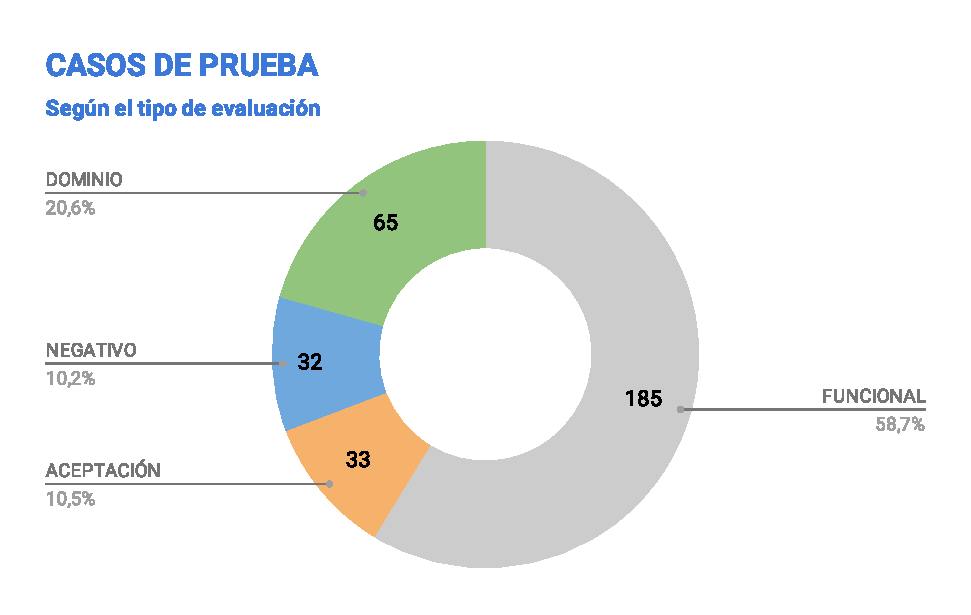
\includegraphics[width=1.0\textwidth]{graphics/tc-tests.eps}
\caption{Casos de Prueba según el tipo de evaluación realizada.}
\label{tc-tests}
\source{Elaboración propia.}
\end{figure}

\begin{figure}
\centering
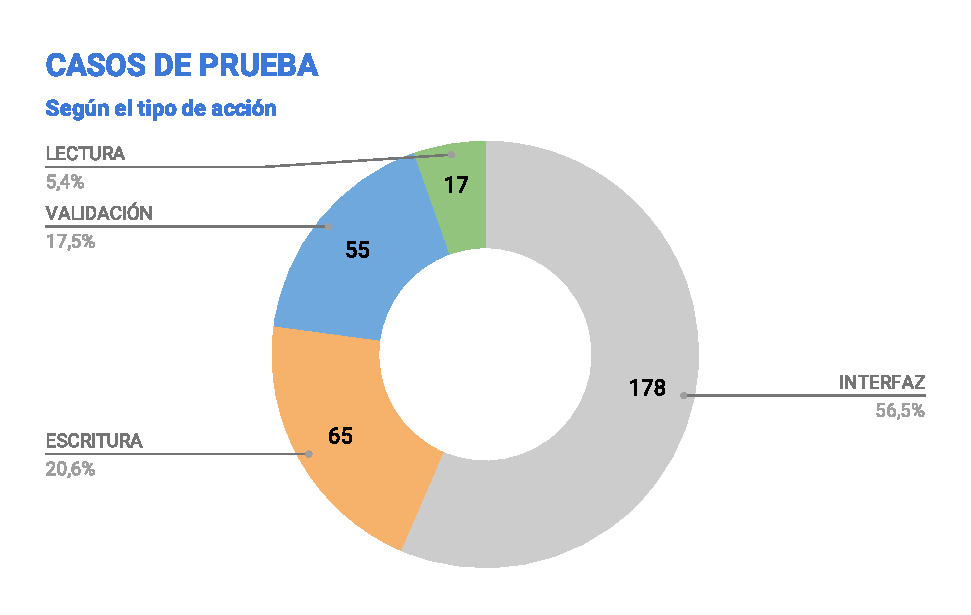
\includegraphics[width=1.0\textwidth]{graphics/tc-type.eps}
\caption{Casos de Prueba según el tipo de acción a evaluar.}
\label{tc-type}
\source{Elaboración propia.}
\end{figure}


\chapter{Desarrollo del Framework}

En este capitulo, trataremos los asuntos concernientes a la construcción de las
funciones del framework, sobre las que recaen la automatización de los casos de
prueba, y la expansibilidad que pueda darse a todo el proyecto.

Si bien en el anterior capitulo el tema fundamental era el análisis y
exploración que se realizo sobre el software, el objeto central de este
capitulo es el framework mismo.

\section{Casos de prueba}
A partir del análisis realizado en el anterior capitulo, se termino formulando
múltiples casos de prueba, estos se encuentran descritos en el \textbf{apéndice
\ref{appendix}} categorizados e individualizados según el área y suba rea al que
pertenecen.

\section{Código fuente}
Todo el código fuente del framework se encuentra versionado y disponible desde
github, en la siguiente dirección:
\\
\\
\centerline{\textbf{https://github.com/ccaballero/salesforce\_automation}}

\section{Estructura del Framework}
El framework desarrollado basa su estructura y comportamiento en las
recomendaciones de la biblioteca utilizada (\emph{webdriver.io}), esta puede
verse en la figura \ref{structura}.

\begin{figure}
\centering

\includegraphics[width=1.0\textwidth]{graphics/diagram00.eps}
\caption{Estructura de archivos del Framework.}
\label{structura}
\end{figure}

Puede observarse en esta figura, que se creó la carpeta \textbf{/PageObjects}
para albergar todas las clases que representan elementos de las paginas que
componen el framework, además de una carpeta \textbf{/Specs} que alberga los
casos de prueba automatizados, adicionalmente existe la carpeta \textbf{Utils}
donde se ubicaron Clases adicionales utilitarias.

Adicionalmente a estas carpetas también se encuentran los ficheros relacionados
con la biblioteca webdriver.io, utilizados como se detallan a continuación:

\begin{description}
\item [config.dist.js] Archivo de configuración del framework, sin
    credenciales para ser versionado con el sistema de control de cambios.
\item [config.js] Archivo de configuración del framework, donde están
    parametrizados todas las variables y credenciales necesarias durante la
    ejecución.
\item [docker-compose.yml] Archivo de orquestación de imágenes utilizados para
    la ejecución de los casos de prueba sobre imágenes de \emph{Docker}.
\item [package.json] Archivo de configuración de node.js, que incluye los
    diferentes tipos de ejecución disponible, las bibliotecas utilizadas, entre
    otros detalles menores acerca del proyecto.
\item [wdio.browserstack.conf.js] Archivo de configuración utilizado por la
    biblioteca \emph{webdriver.io} para la ejecución de las pruebas sobre el
    servicio \emph{BrowserStack}.
\item [wdio.conf.js] Archivo de configuración de \emph{webdriver.io}, este
    contiene las conjuntos de pruebas disponibles, entre otras variables
    utilizadas por el entorno de prueba.
\item [wdio.docker.conf.js] Archivo de configuración utilizado por la
    biblioteca \emph{webdriver.io} para la ejecución de las pruebas sobre el
    servidor \emph{Docker}.
\item [wdio.standalone.conf.js] Archivo de configuración utilizado por la
    biblioteca \emph{webdriver.io} para la ejecución de las pruebas sobre el
    mismo ordenador en modo solitario.
\end{description}

\section{Suites Disponibles}
El proyecto ha sido configurado de forma que puedan ejecutarse diferentes
conjuntos de casos de prueba, estos se detallan en el cuadro \ref{suites}.

\begin{table}
\centering
\begin{tabular}{|l|p{12.0cm}|}
\hline
\footnotesize{\textbf{Suite}} & \footnotesize{\textbf{Descripción}} \\
\hline
\footnotesize{\emph{init}} & \footnotesize{Ejecución de una prueba rápida de
disponibilidad de la URL principal de \emph{Salesforce} a evaluar.} \\
\footnotesize{\emph{login}} & \footnotesize{Ejecución de una prueba rápida de
acceso al sistema, útil para verificación de credenciales.} \\
\footnotesize{\emph{products}} & \footnotesize{Ejecución de todos los casos de
prueba relacionados con el modulo de gestión  de productos.} \\
\footnotesize{\emph{pricebooks}} & \footnotesize{Ejecución de todos los casos de
prueba relacionados con el modulo de gestión de listas de precios.} \\
\footnotesize{\emph{listviews}} & \footnotesize{Ejecución de todos los casos de
prueba relacionados con el modulo de gestión de vistas de listas.} \\
\footnotesize{\emph{functional}} & \footnotesize{Ejecución de todos los casos de
prueba relacionados con pruebas funcionales en todos los módulos.} \\
\footnotesize{\emph{acceptance}} & \footnotesize{Ejecución de todos los casos de
prueba relacionados con pruebas de aceptación en todos los módulos.} \\
\footnotesize{\emph{negative}} & \footnotesize{Ejecución de todos los casos de
prueba relacionados con pruebas negativas en todos los módulos.} \\
\footnotesize{\emph{domain}} & \footnotesize{Ejecución de todos los casos de
prueba relacionados con pruebas de dominio en todos los módulos.} \\
\hline
\end{tabular}
\caption{Ediciones actualmente disponibles de \emph{Sales Cloud}.}
\label{suites}
\end{table}

\section{\emph{Page Objects Model}}
Los \emph{Page Objects} representan el corazón del proyecto de automatización,
estos representan las diferentes paginas a ser testeadas y algunos de sus
componentes que posean cierto grado de complejidad.

Si bien los \emph{Page Objects} son clases instanciables en \emph{javascript},
la mayor parte son utilizados de manera estática y con un relacionamiento
entre estos que es dinámico y sustancialmente inexistente, aun así puede
utilizarse un diagrama de clases convencional para comprender las relaciones
entre estos como se presenta en la figura \ref{pom}.

\begin{figure}
\centering

\includegraphics[width=1.0\textwidth]{graphics/diagram00.eps}
\caption{Diagrama de clases sobre las relaciones entre \emph{Page Objects}.}
\label{pom}
\end{figure}

\section{\emph{Specs}}
Los \emph{Specs} representan las rutinas de automatización propiamente dichas,
en estas se encuentran la implementación de los casos de prueba; para el
proyecto se ha intentando hacer de estos lo mas expresivos posibles de forma
que su legibilidad sea la mayor, por ejemplo puede apreciarse en la figura
\ref{spec} que referencia al caso de prueba A001.

\begin{figure}
\centering

\includegraphics[width=1.0\textwidth]{graphics/diagram00.eps}
\caption{\emph{Spec} que cubre el caso de prueba A001.}
\label{spec}
\end{figure}

Este \emph{spec} que cubre la automatización del caso de prueba A001, utiliza
cinco \emph{page objects}, dos utilizadas para la ejecución de las
precondiciones del test, y tres para realizar la secuencia de pasos, como puede
verse en el diagrama de secuencia de la figura \ref{sequence}.

\begin{figure}
\centering

\includegraphics[width=1.0\textwidth]{graphics/diagram00.eps}
\caption{Diagrama de secuencia para el \emph{spec} del caso de prueba A001.}
\label{sequence}
\end{figure}

\section{Ejecución de las pruebas}
En la figura \ref{tc-tests}, se puede ver la distribución de los casos de prueba
según el tipo de evaluación realizado, puede apreciarse que las pruebas
funcionales ocupan mas de la mitad de la totalidad de casos de prueba en el
proyecto, mientras que los casos de prueba negativos, y de aceptación, están más
próximos al 10\%.

En la figura \ref{tc-type}, se puede ver la distribución de los casos de prueba
según el tipo de acción que se realiza en el sistema, es decir, si son casos
que afectan la interfaz de usuario, si mas bien son funciones de validación, o
si realizan alguna petición al servidor, sea esta de lectura o escritura.

\begin{figure}[H]
\centering
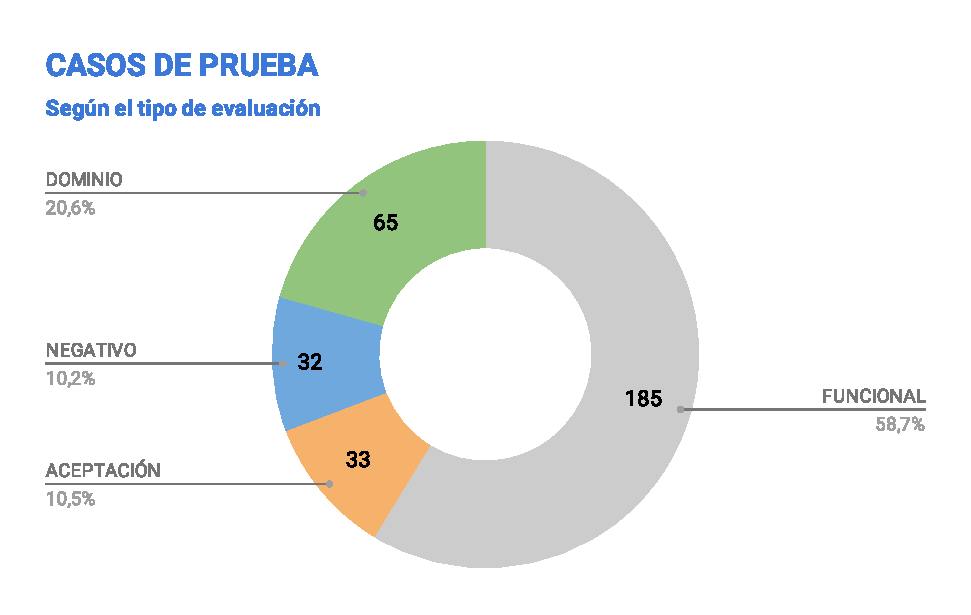
\includegraphics[width=1.0\textwidth]{graphics/tc-tests.eps}
\caption{Casos de Prueba según el tipo de evaluación realizada.}
\label{tc-tests}
\end{figure}

\begin{figure}[H]
\centering
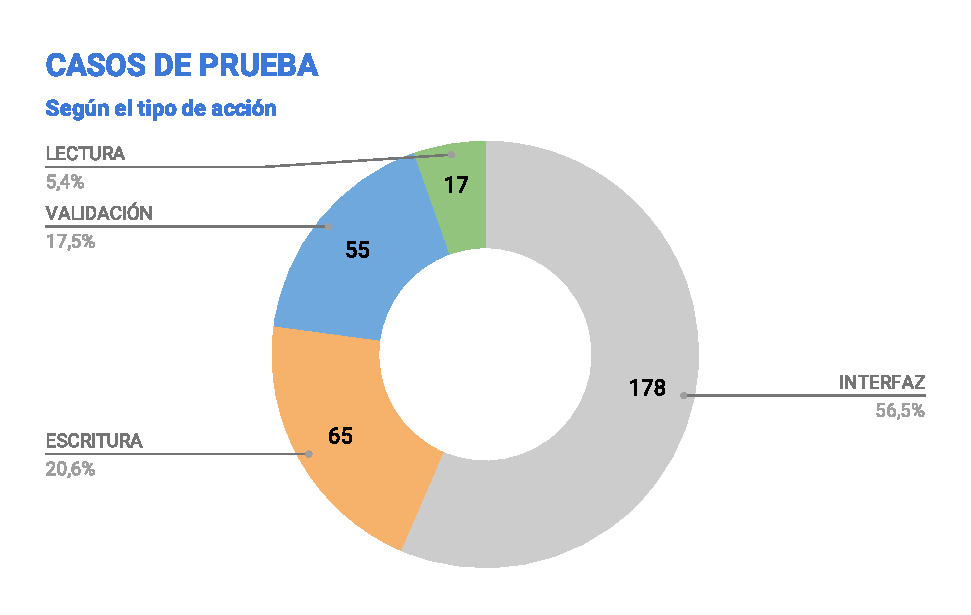
\includegraphics[width=1.0\textwidth]{graphics/tc-type.eps}
\caption{Casos de Prueba según el tipo de acción a evaluar.}
\label{tc-type}
\end{figure}

Puede apreciarse igualmente que la mayor parte de los casos de prueba están
orientados a evaluar el comportamiento de la interfaz de usuario, mientras que
en un 25\% aproximadamente se evalúan funcionalidades que se comunican con el
servidor.

En las figuras \ref{results-tests} y \ref{results-type}, se condensan los
resultados obtenidos de la ejecución de los casos de prueba, en los cuales
únicamente fallaron 2 casos de prueba, ambos relacionados a un mismo formulario,
como puede verse en el reporte de error adjunto, y debido al fallo de estos
también se bloquearon dos casos de prueba.

\begin{figure}[H]
\centering
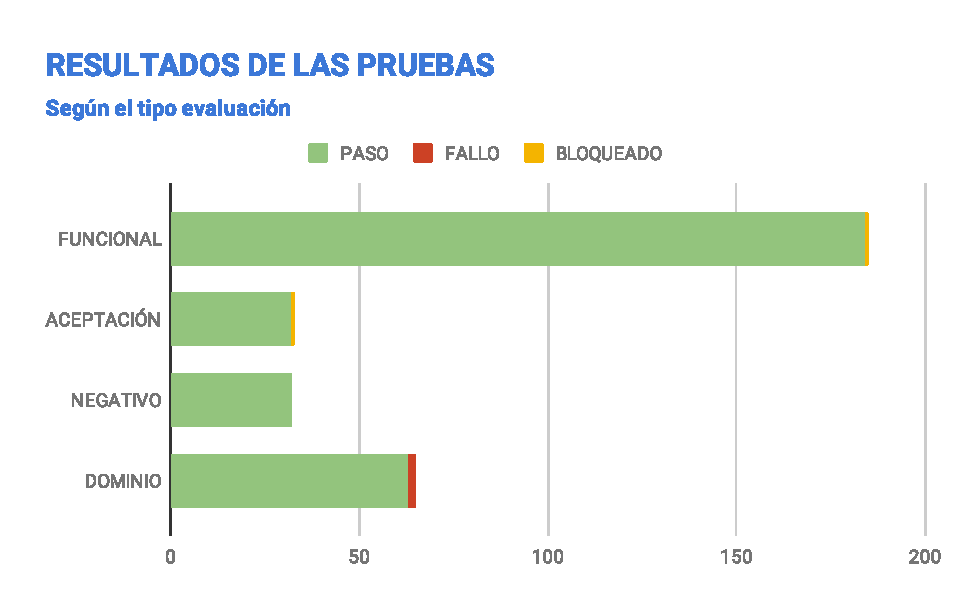
\includegraphics[width=1.0\textwidth]{graphics/results-tests.eps}
\caption{Resultados de las pruebas clasificadas por tipo de evaluación.}
\label{results-tests}
\end{figure}

\begin{figure}[H]
\centering
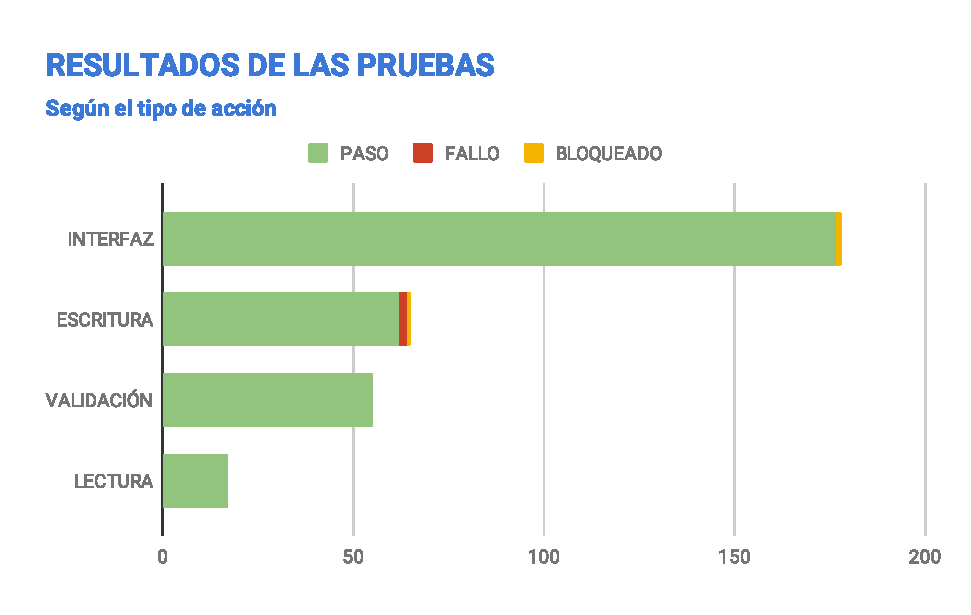
\includegraphics[width=1.0\textwidth]{graphics/results-type.eps}
\caption{Resultados de las pruebas clasificadas por tipo de acción a evaluar.}
\label{results-type}
\end{figure}

Presentados los resultados de la ejecución de las pruebas, vemos que de los 315
casos de pruebas únicamente existen 2 bloqueados, y dos fallidos. Por ende se
tiene 98.74\% de casos de prueba exitosos, lo que lleva a concluir que los
atributos de calidad esperados del sistema están cubiertos por completo.



\begin{appendix}
\chapter{Casos de prueba}
\label{appendix_testscases}
Este apéndice tiene como objetivo citar los casos de prueba formulados para el
proyecto, clasificados por el tipo de evaluación que ha sido ejecutado y el tipo
de acción que se esta evaluando.

Para la compresión de las tablas es necesario tener en cuenta las siguientes
abreviaturas:

\begin{itemize}
    \item P, hace referencia al modulo de Productos.
    \item LP, hace referencia al modulo de Listas de Precios.
    \item VL, hace referencia al componente de Vistas de Lista.
    \item A00x, es el modelo de ID para un caso de prueba de tipo aceptación.
    \item F00x, es el modelo de ID para un caso de prueba de tipo funcional.
    \item D00x, es el modelo de ID para un caso de prueba de tipo dominio.
    \item N00x, es el modelo de ID para un caso de prueba de tipo negativo.
\end{itemize}

\begin{landscape}
\centering
\small
{\def\arraystretch{1}
\begin{longtable}[htb]{|c|c|p{3.8cm}|p{15.2cm}|}
\hline
\scriptsize{\textbf{ID}} & \scriptsize{\textbf{Área}} &
\scriptsize{\textbf{Subarea}} & \scriptsize{\textbf{Caso de Prueba}} \\
\hline
\scriptsize{F001} & \scriptsize{P} & & \scriptsize{Iniciador de Aplicación de Salesforce muestra el enlace a «Productos»} \\ \hline
\scriptsize{F002} & \scriptsize{P} & \scriptsize{NUEVO} & \scriptsize{Clic en el botón «Nuevo», lanza el formulario de creación de producto} \\ \hline
\scriptsize{A001} & \scriptsize{P} & \scriptsize{NUEVO} & \scriptsize{Producto es registrado con los valores obligatorios establecidos después de accionado el botón «Guardar»} \\ \hline
\scriptsize{F003} & \scriptsize{P} & \scriptsize{NUEVO} & \scriptsize{Producto es registrado con los valores obligatorios establecidos después de accionado el botón «Guardar y nuevo»} \\ \hline
\scriptsize{F004} & \scriptsize{P} & \scriptsize{NUEVO} & \scriptsize{Formulario «Crear Producto» se cierra al accionar el botón «Cancelar»} \\ \hline
\scriptsize{F005} & \scriptsize{P} & \scriptsize{NUEVO} & \scriptsize{Formulario «Crear Producto» se cierra al accionar el botón «Cerrar esta ventana (X)»} \\ \hline
\scriptsize{N001} & \scriptsize{P} & \scriptsize{NUEVO} & \scriptsize{Clic en el botón «Guardar» para un formulario vacío envía el mensaje «Revise los errores de esta página»} \\ \hline
\scriptsize{F006} & \scriptsize{P} & \scriptsize{NUEVO} & \scriptsize{Mensaje «Se creó Producto "$<$Nombre de Producto$>$"» se muestra después de registrado un producto} \\ \hline
\scriptsize{D001} & \scriptsize{P} & \scriptsize{NUEVO-FORMULARIO} & \scriptsize{Formulario «Crear Producto» no realiza el registro, cuando el campo «Nombre del producto» tiene 0 caracteres} \\ \hline
\scriptsize{D002} & \scriptsize{P} & \scriptsize{NUEVO-FORMULARIO} & \scriptsize{Formulario «Crear Producto» realiza el registro, cuando el campo «Nombre del producto» tiene 1 carácter} \\ \hline
\scriptsize{D003} & \scriptsize{P} & \scriptsize{NUEVO-FORMULARIO} & \scriptsize{Formulario «Crear Producto» realiza el registro, cuando el campo «Nombre del producto» tiene 255 caracteres} \\ \hline
\scriptsize{D004} & \scriptsize{P} & \scriptsize{NUEVO-FORMULARIO} & \scriptsize{Formulario «Crear Producto» no realiza el registro, cuando el campo «Nombre del producto» tiene 256 caracteres} \\ \hline
\scriptsize{D005} & \scriptsize{P} & \scriptsize{NUEVO-FORMULARIO} & \scriptsize{Formulario «Crear Producto» realiza el registro, cuando el campo «Código del producto» tiene 0 caracteres} \\ \hline
\scriptsize{D006} & \scriptsize{P} & \scriptsize{NUEVO-FORMULARIO} & \scriptsize{Formulario «Crear Producto» realiza el registro, cuando el campo «Código del producto» tiene 255 caracteres} \\ \hline
\scriptsize{D007} & \scriptsize{P} & \scriptsize{NUEVO-FORMULARIO} & \scriptsize{Formulario «Crear Producto» no realiza el registro, cuando el campo «Código del producto» tiene 256 caracteres} \\ \hline
\scriptsize{D008} & \scriptsize{P} & \scriptsize{NUEVO-FORMULARIO} & \scriptsize{Formulario «Crear Producto» realiza el registro, cuando el campo «Descripción del producto» tiene 0 caracteres} \\ \hline
\scriptsize{D009} & \scriptsize{P} & \scriptsize{NUEVO-FORMULARIO} & \scriptsize{Formulario «Crear Producto» realiza el registro, cuando el campo «Descripción del producto» tiene 4000 caracteres} \\ \hline
\scriptsize{D010} & \scriptsize{P} & \scriptsize{NUEVO-FORMULARIO} & \scriptsize{Formulario «Crear Producto» no realiza el registro, cuando el campo «Descripción del producto» tiene 4001 caracteres} \\ \hline
\scriptsize{F007} & \scriptsize{P} & \scriptsize{BUSCAR} & \scriptsize{«Buscar en esta lista...» filtra los elementos a partir de contenido en el campo «Nombre del producto»} \\ \hline
\scriptsize{F008} & \scriptsize{P} & \scriptsize{BUSCAR} & \scriptsize{«Buscar en esta lista...» filtra los elementos a partir de contenido en el campo «Código de producto»} \\ \hline
\scriptsize{F009} & \scriptsize{P} & \scriptsize{BUSCAR} & \scriptsize{«Buscar en esta lista...» filtra los elementos a partir de contenido en el campo «Descripción de producto»} \\ \hline
\scriptsize{N002} & \scriptsize{P} & \scriptsize{BUSCAR} & \scriptsize{Mensaje «No hay elementos para mostrar» se muestra cuando la búsqueda no presenta resultados} \\ \hline
\scriptsize{F010} & \scriptsize{P} & \scriptsize{MOSTRAR COMO} & \scriptsize{«Mostrar como» posee los elementos: «Tabla» y «Kanban»} \\ \hline
\scriptsize{F011} & \scriptsize{P} & \scriptsize{MOSTRAR COMO} & \scriptsize{Opción «Tabla» en «Mostrar como», muestra los productos en formato tabular} \\ \hline
\scriptsize{F012} & \scriptsize{P} & \scriptsize{MOSTRAR COMO} & \scriptsize{Opción «Kanban» en «Mostrar como», muestra los productos en formato de columnas} \\ \hline
\scriptsize{F013} & \scriptsize{P} & \scriptsize{ACTUALIZAR} & \scriptsize{Botón «Actualizar», reenvía las peticiones de consulta al servidor} \\ \hline
\scriptsize{N003} & \scriptsize{P} & \scriptsize{MOSTRAR GRÁFICOS} & \scriptsize{«Mostrar Gráficos» está deshabilitado mientras no se use una «vista de lista» determinada} \\ \hline
\scriptsize{F014} & \scriptsize{P} & \scriptsize{MOSTRAR GRÁFICOS} & \scriptsize{«Mostrar Gráficos» está habilitado mientras se use una «vista de lista» determinada} \\ \hline
\scriptsize{N004} & \scriptsize{P} & \scriptsize{MOSTRAR FILTROS} & \scriptsize{«Mostrar filtros» está deshabilitado mientras no se use una «vista de lista» determinada} \\ \hline
\scriptsize{F015} & \scriptsize{P} & \scriptsize{MOSTRAR FILTROS} & \scriptsize{«Mostrar filtros» está habilitado mientras se use una «vista de lista» determinada} \\ \hline
\scriptsize{F016} & \scriptsize{P} & \scriptsize{FILTRAR} & \scriptsize{«Vistas de Lista» muestra los elementos registrados} \\ \hline
\scriptsize{F017} & \scriptsize{P} & \scriptsize{FILTRAR} & \scriptsize{«Vistas de Lista» muestra el elemento «Vistos recientemente»} \\ \hline
\scriptsize{N005} & \scriptsize{P} & \scriptsize{FILTRAR} & \scriptsize{Mensaje «No hay elementos para mostrar» se muestra cuando no existen productos bajo una vista de lista} \\ \hline
\scriptsize{F018} & \scriptsize{P} & \scriptsize{FILTRAR} & \scriptsize{Activar un «Vista de Lista» creada, filtra los productos basados en sus criterios establecidos} \\ \hline
\scriptsize{A002} & \scriptsize{P} & \scriptsize{LISTA} & \scriptsize{Vista de Lista «Vistos recientemente» lista los productos registrados} \\ \hline
\scriptsize{N006} & \scriptsize{P} & \scriptsize{LISTA} & \scriptsize{Mensaje «No hay elementos para mostrar» cuando ningún producto ha sido registrado} \\ \hline
\scriptsize{F019} & \scriptsize{P} & \scriptsize{LISTA} & \scriptsize{Columnas en la tabla de productos pueden reordenar la lista dinámicamente} \\ \hline
\scriptsize{F020} & \scriptsize{P} & \scriptsize{LISTA} & \scriptsize{Columnas en la tabla de productos permiten «Ajustar Texto»} \\ \hline
\scriptsize{F021} & \scriptsize{P} & \scriptsize{LISTA} & \scriptsize{Columnas en la tabla de productos permiten «Recortar Texto»} \\ \hline
\scriptsize{F022} & \scriptsize{P} & \scriptsize{LISTA} & \scriptsize{Tabla de productos permite la selección múltiple de elementos} \\ \hline
\scriptsize{F023} & \scriptsize{P} & \scriptsize{LISTA} & \scriptsize{Tabla de productos ofrece selección y de-selección de todos los elementos} \\ \hline
\scriptsize{F024} & \scriptsize{P} & \scriptsize{LISTA} & \scriptsize{Elementos de la tabla de productos ofrecen un enlace para «Ver»} \\ \hline
\scriptsize{F025} & \scriptsize{P} & \scriptsize{LISTA} & \scriptsize{Elementos de la tabla de productos ofrecen un enlace para «Modificar»} \\ \hline
\scriptsize{F026} & \scriptsize{P} & \scriptsize{LISTA} & \scriptsize{Elementos de la tabla de productos ofrecen un enlace para «Eliminar»} \\ \hline
\scriptsize{F027} & \scriptsize{P} & \scriptsize{LISTA} & \scriptsize{Celdas de la tabla de productos pueden ser editados} \\ \hline
\scriptsize{F028} & \scriptsize{P} & \scriptsize{LISTA} & \scriptsize{Tabla de productos muestra la Opción «Guardar» cuando existen elementos editados} \\ \hline
\scriptsize{F029} & \scriptsize{P} & \scriptsize{LISTA} & \scriptsize{Tabla de productos muestra la Opción «Cancelar» cuando existen elementos editados} \\ \hline
\scriptsize{F030} & \scriptsize{P} & \scriptsize{LISTA} & \scriptsize{Elementos editados en la tabla de productos solicitan confirmación de descarte antes de cambiar de vista} \\ \hline
\scriptsize{A003} & \scriptsize{P} & \scriptsize{LISTA} & \scriptsize{Tabla de productos registra la información modificada de las celdas editadas} \\ \hline
\scriptsize{F031} & \scriptsize{P} & \scriptsize{VER} & \scriptsize{Vista de producto muestra las opciones de «Modificar», «Eliminar», y «Duplicar»} \\ \hline
\scriptsize{A004} & \scriptsize{P} & \scriptsize{VER-DETALLES} & \scriptsize{Vista de producto muestra la información del producto en su pestaña «Detalles»} \\ \hline
\scriptsize{A005} & \scriptsize{P} & \scriptsize{VER-RELACIONADO} & \scriptsize{Vista de producto muestra la lista de «Listas de precios» en su pestaña «Relacionado»} \\ \hline
\scriptsize{F032} & \scriptsize{P} & \scriptsize{VER-RELACIONADO} & \scriptsize{«Agregar precio estándar» es visible cuando el producto no tiene un precio establecido} \\ \hline
\scriptsize{N007} & \scriptsize{P} & \scriptsize{VER-RELACIONADO} & \scriptsize{«Agregar precio estándar» no es visible cuando el producto tiene un precio establecido} \\ \hline
\scriptsize{F033} & \scriptsize{P} & \scriptsize{VER-RELACIONADO} & \scriptsize{Clic en el botón «Agregar precio estándar», lanza el formulario de creación de entrada del catálogo de precios} \\ \hline
\scriptsize{A006} & \scriptsize{P} & \scriptsize{VER-RELACIONADO} & \scriptsize{Precio estándar del producto es registrado con un valor de 1 después de accionado el botón «Guardar»} \\ \hline
\scriptsize{F034} & \scriptsize{P} & \scriptsize{VER-RELACIONADO} & \scriptsize{Precio estándar del producto es registrado con un valor de 1 después de accionado el botón «Guardar y nuevo»} \\ \hline
\scriptsize{F035} & \scriptsize{P} & \scriptsize{VER-RELACIONADO} & \scriptsize{Formulario «Crear Entrada del catálogo de precios» se cierra al accionar el botón «Cancelar»} \\ \hline
\scriptsize{F036} & \scriptsize{P} & \scriptsize{VER-RELACIONADO} & \scriptsize{Formulario «Crear Entrada del catálogo de precios» se cierra al accionar el botón «Cerrar esta ventana (X)»} \\ \hline
\scriptsize{N008} & \scriptsize{P} & \scriptsize{VER-RELACIONADO} & \scriptsize{Clic en el botón «Guardar» para un formulario vacío envía el mensaje «Revise los errores de esta página»} \\ \hline
\scriptsize{F037} & \scriptsize{P} & \scriptsize{VER-RELACIONADO} & \scriptsize{Mensaje «Se creó Entrada del catálogo de precios ."» se muestra después de registrado un precio estándar} \\ \hline
\scriptsize{D011} & \scriptsize{P} & \scriptsize{VER-RELACIONADO-FORMULARIO} & \scriptsize{Formulario «Crear Entrada del catálogo de precios» no permite el registro, cuando en el campo «Precio de la lista» se ingresa el valor -9.007.199.254.740.992} \\ \hline
\scriptsize{D012} & \scriptsize{P} & \scriptsize{VER-RELACIONADO-FORMULARIO} & \scriptsize{Formulario «Crear Entrada del catálogo de precios» permite el registro, cuando en el campo «Precio de la lista» se ingresa el valor -9.007.199.254.740.991} \\ \hline
\scriptsize{D013} & \scriptsize{P} & \scriptsize{VER-RELACIONADO-FORMULARIO} & \scriptsize{Formulario «Crear Entrada del catálogo de precios» no permite el registro, cuando en el campo «Precio de la lista» se ingresa el valor 0,9999} \\ \hline
\scriptsize{D014} & \scriptsize{P} & \scriptsize{VER-RELACIONADO-FORMULARIO} & \scriptsize{Formulario «Crear Entrada del catálogo de precios» permite el registro, cuando en el campo «Precio de la lista» se ingresa el valor 0,999} \\ \hline
\scriptsize{D015} & \scriptsize{P} & \scriptsize{VER-RELACIONADO-FORMULARIO} & \scriptsize{Formulario «Crear Entrada del catálogo de precios» permite el registro, cuando en el campo «Precio de la lista» se ingresa el valor 9.007.199.254.740.991} \\ \hline
\scriptsize{D016} & \scriptsize{P} & \scriptsize{VER-RELACIONADO-FORMULARIO} & \scriptsize{Formulario «Crear Entrada del catálogo de precios» no permite el registro, cuando en el campo «Precio de la lista» se ingresa el valor 9.007.199.254.740.992} \\ \hline
\scriptsize{F038} & \scriptsize{P} & \scriptsize{VER-RELACIONADO} & \scriptsize{Clic en el botón «Agregar a lista de precios», lanza el formulario de agregar a lista de precios} \\ \hline
\scriptsize{A007} & \scriptsize{P} & \scriptsize{VER-RELACIONADO} & \scriptsize{Precio de producto para una lista de precios es registrado después de accionado el botón «Guardar»} \\ \hline
\scriptsize{F039} & \scriptsize{P} & \scriptsize{VER-RELACIONADO} & \scriptsize{Formulario «Agregar a lista de precios» se cierra al accionar el botón «Cancelar»} \\ \hline
\scriptsize{F040} & \scriptsize{P} & \scriptsize{VER-RELACIONADO} & \scriptsize{Formulario «Agregar a lista de precios» se cierra al accionar el botón «Cerrar esta ventana (X)»} \\ \hline
\scriptsize{N009} & \scriptsize{P} & \scriptsize{VER-RELACIONADO} & \scriptsize{Clic en el botón «Siguiente» para un formulario vacío envía el mensaje «Revise los errores de esta página»} \\ \hline
\scriptsize{F041} & \scriptsize{P} & \scriptsize{VER-RELACIONADO} & \scriptsize{Mensaje «Se guardó Entrada del catálogo de precios ."» se muestra después de modificado un precio} \\ \hline
\scriptsize{D017} & \scriptsize{P} & \scriptsize{VER-RELACIONADO-FORMULARIO} & \scriptsize{Formulario «Agregar a lista de precios» permite el registro, cuando en el campo «Lista de precios» se ingresa el valor Nulo} \\ \hline
\scriptsize{D018} & \scriptsize{P} & \scriptsize{VER-RELACIONADO-FORMULARIO} & \scriptsize{Formulario «Agregar a lista de precios» permite el registro, cuando en el campo «Divisa» se ingresa el valor Nulo} \\ \hline
\scriptsize{F042} & \scriptsize{P} & \scriptsize{VER-RELACIONADO-LISTA} & \scriptsize{Elementos de la lista de «Listas de precios» ofrecen un enlace para «Ver»} \\ \hline
\scriptsize{F043} & \scriptsize{P} & \scriptsize{VER-RELACIONADO-LISTA} & \scriptsize{Elementos de la lista de «Listas de precios» ofrecen un enlace para «Modificar»} \\ \hline
\scriptsize{F044} & \scriptsize{P} & \scriptsize{VER-RELACIONADO-LISTA} & \scriptsize{Elementos de la lista de «Listas de precios» ofrecen un enlace para «Eliminar»} \\ \hline
\scriptsize{F045} & \scriptsize{P} & \scriptsize{VER-RELACIONADO-LISTA-MODIFICAR} & \scriptsize{Clic en el botón «Modificar», lanza el formulario «Modificar Entrada del catálogo de precios»} \\ \hline
\scriptsize{A008} & \scriptsize{P} & \scriptsize{VER-RELACIONADO-LISTA-MODIFICAR} & \scriptsize{Precio del producto es modificado con los valores obligatorios establecidos después de accionado el botón «Guardar»} \\ \hline
\scriptsize{F046} & \scriptsize{P} & \scriptsize{VER-RELACIONADO-LISTA-MODIFICAR} & \scriptsize{Precio del producto es modificado con los valores obligatorios establecidos después de accionado el botón «Guardar y nuevo»} \\ \hline
\scriptsize{F047} & \scriptsize{P} & \scriptsize{VER-RELACIONADO-LISTA-MODIFICAR} & \scriptsize{Formulario «Modificar Entrada del catálogo de precios» se cierra al accionar el botón «Cancelar»} \\ \hline
\scriptsize{F048} & \scriptsize{P} & \scriptsize{VER-RELACIONADO-LISTA-MODIFICAR} & \scriptsize{Formulario «Modificar Entrada del catálogo de precios» se cierra al accionar el botón «Cerrar esta ventana (X)»} \\ \hline
\scriptsize{F049} & \scriptsize{P} & \scriptsize{VER-RELACIONADO-LISTA-MODIFICAR} & \scriptsize{Formulario «Modificar Entrada del catálogo de precios» no permite marcar «Utilizar Precio estándar» en la lista de precios por defecto} \\ \hline
\scriptsize{N010} & \scriptsize{P} & \scriptsize{VER-RELACIONADO-LISTA-MODIFICAR} & \scriptsize{Formulario «Modificar Entrada del catálogo de precios» permite marcar «Utilizar Precio estándar» en la lista de precios que no son por defecto} \\ \hline
\scriptsize{N011} & \scriptsize{P} & \scriptsize{VER-RELACIONADO-LISTA-MODIFICAR} & \scriptsize{Clic en el botón «Guardar» para un formulario vacío envía el mensaje «Revise los errores de esta página»} \\ \hline
\scriptsize{F050} & \scriptsize{P} & \scriptsize{VER-RELACIONADO-LISTA-MODIFICAR} & \scriptsize{Mensaje «Se guardó Entrada del catálogo de precios ."» se muestra después de modificado un precio} \\ \hline
\scriptsize{D019} & \scriptsize{P} & \scriptsize{VER-RELACIONADO-LISTA-MODIFICAR} & \scriptsize{Formulario «Modificar Entrada del catálogo de precios» no permite el registro, cuando en el campo «Precio de la lista» se ingresa el valor -9.007.199.254.740.992} \\ \hline
\scriptsize{D020} & \scriptsize{P} & \scriptsize{VER-RELACIONADO-LISTA-MODIFICAR} & \scriptsize{Formulario «Modificar Entrada del catálogo de precios» permite el registro, cuando en el campo «Precio de la lista» se ingresa el valor -9.007.199.254.740.991} \\ \hline
\scriptsize{D021} & \scriptsize{P} & \scriptsize{VER-RELACIONADO-LISTA-MODIFICAR} & \scriptsize{Formulario «Modificar Entrada del catálogo de precios» no permite el registro, cuando en el campo «Precio de la lista» se ingresa el valor 0,9999} \\ \hline
\scriptsize{D022} & \scriptsize{P} & \scriptsize{VER-RELACIONADO-LISTA-MODIFICAR} & \scriptsize{Formulario «Modificar Entrada del catálogo de precios» permite el registro, cuando en el campo «Precio de la lista» se ingresa el valor 0,999} \\ \hline
\scriptsize{D023} & \scriptsize{P} & \scriptsize{VER-RELACIONADO-LISTA-MODIFICAR} & \scriptsize{Formulario «Modificar Entrada del catálogo de precios» permite el registro, cuando en el campo «Precio de la lista» se ingresa el valor 9.007.199.254.740.991} \\ \hline
\scriptsize{D024} & \scriptsize{P} & \scriptsize{VER-RELACIONADO-LISTA-MODIFICAR} & \scriptsize{Formulario «Modificar Entrada del catálogo de precios» no permite el registro, cuando en el campo «Precio de la lista» se ingresa el valor 9.007.199.254.740.992} \\ \hline
\scriptsize{F051} & \scriptsize{P} & \scriptsize{VER-RELACIONADO-LISTA-MODIFICAR-CREAR} & \scriptsize{Botón «Guardar y nuevo» muestra el formulario «Crear Entrada del catálogo de precios»} \\ \hline
\scriptsize{A009} & \scriptsize{P} & \scriptsize{VER-RELACIONADO-LISTA-MODIFICAR-CREAR} & \scriptsize{Precio del producto es modificado con los valores obligatorios establecidos después de accionado el botón «Guardar»} \\ \hline
\scriptsize{F052} & \scriptsize{P} & \scriptsize{VER-RELACIONADO-LISTA-MODIFICAR-CREAR} & \scriptsize{Precio del producto es modificado con los valores obligatorios establecidos después de accionado el botón «Guardar y nuevo»} \\ \hline
\scriptsize{F053} & \scriptsize{P} & \scriptsize{VER-RELACIONADO-LISTA-MODIFICAR-CREAR} & \scriptsize{Formulario «Crear Entrada del catálogo de precios» se cierra al accionar el botón «Cancelar»} \\ \hline
\scriptsize{F054} & \scriptsize{P} & \scriptsize{VER-RELACIONADO-LISTA-MODIFICAR-CREAR} & \scriptsize{Formulario «Crear Entrada del catálogo de precios» se cierra al accionar el botón «Cerrar esta ventana (X)»} \\ \hline
\scriptsize{N012} & \scriptsize{P} & \scriptsize{VER-RELACIONADO-LISTA-MODIFICAR-CREAR} & \scriptsize{Clic en el botón «Guardar» para un formulario vacío envía el mensaje «Revise los errores de esta página»} \\ \hline
\scriptsize{F055} & \scriptsize{P} & \scriptsize{VER-RELACIONADO-LISTA-MODIFICAR-CREAR} & \scriptsize{Mensaje «Se creó Entrada del catálogo de precios ."» se muestra después de modificado un precio} \\ \hline
\scriptsize{F056} & \scriptsize{P} & \scriptsize{VER-RELACIONADO-LISTA-ELIMINAR} & \scriptsize{Clic en el botón «Eliminar», lanza un mensaje de confirmación} \\ \hline
\scriptsize{A010} & \scriptsize{P} & \scriptsize{VER-RELACIONADO-LISTA-ELIMINAR} & \scriptsize{Precio es eliminado después de accionado el botón «Eliminar»} \\ \hline
\scriptsize{N013} & \scriptsize{P} & \scriptsize{VER-RELACIONADO-LISTA-ELIMINAR} & \scriptsize{Precio estándar no puede ser eliminado después de accionado el botón «Eliminar», si existen referencias en otras listas de precios} \\ \hline
\scriptsize{F057} & \scriptsize{P} & \scriptsize{VER-RELACIONADO-LISTA-ELIMINAR} & \scriptsize{Confirmación «Eliminar Entrada del catálogo de precios» se cierra al accionar el botón «Cancelar»} \\ \hline
\scriptsize{F058} & \scriptsize{P} & \scriptsize{VER-RELACIONADO-LISTA-ELIMINAR} & \scriptsize{Confirmación «Eliminar Entrada del catálogo de precios» se cierra al accionar el botón «Cerrar esta ventana (X)»} \\ \hline
\scriptsize{F059} & \scriptsize{P} & \scriptsize{VER-RELACIONADO-LISTA-ELIMINAR} & \scriptsize{Mensaje «Se eliminó Producto "$<$Nombre de Producto$>$"» se muestra después de eliminado un producto} \\ \hline
\scriptsize{F060} & \scriptsize{P} & \scriptsize{VER-RELACIONADO} & \scriptsize{Clic en el botón «Ver todos» amplía la lista de Listas de precios} \\ \hline
\scriptsize{F061} & \scriptsize{P} & \scriptsize{VER-RELACIONADO} & \scriptsize{Botón «Actualizar» ubicado en la ampliación de la lista de Listas de precios, reenvía las peticiones de consulta al servidor} \\ \hline
\scriptsize{F062} & \scriptsize{P} & \scriptsize{LISTA-MODIFICAR} & \scriptsize{Clic en el botón «Modificar», lanza el formulario de edición de producto} \\ \hline
\scriptsize{A011} & \scriptsize{P} & \scriptsize{LISTA-MODIFICAR} & \scriptsize{Producto es modificado con los valores obligatorios establecidos después de accionado el botón «Guardar»} \\ \hline
\scriptsize{F063} & \scriptsize{P} & \scriptsize{LISTA-MODIFICAR} & \scriptsize{Producto es modificado con los valores obligatorios establecidos después de accionado el botón «Guardar y nuevo»} \\ \hline
\scriptsize{F064} & \scriptsize{P} & \scriptsize{LISTA-MODIFICAR} & \scriptsize{Formulario de edición de producto se cierra al accionar el botón «Cancelar»} \\ \hline
\scriptsize{F065} & \scriptsize{P} & \scriptsize{LISTA-MODIFICAR} & \scriptsize{Formulario de edición de producto se cierra al accionar el botón «Cerrar esta ventana (X)»} \\ \hline
\scriptsize{N014} & \scriptsize{P} & \scriptsize{LISTA-MODIFICAR} & \scriptsize{Clic en el botón «Guardar» para un formulario vacío envía el mensaje «Revise los errores de esta página»} \\ \hline
\scriptsize{F066} & \scriptsize{P} & \scriptsize{LISTA-MODIFICAR} & \scriptsize{Mensaje «Se guardó Producto "$<$Nombre de Producto$>$"» se muestra después de modificado un producto} \\ \hline
\scriptsize{F067} & \scriptsize{P} & \scriptsize{LISTA-ELIMINAR} & \scriptsize{Clic en el botón «Eliminar», lanza un mensaje de confirmación} \\ \hline
\scriptsize{A012} & \scriptsize{P} & \scriptsize{LISTA-ELIMINAR} & \scriptsize{Producto es eliminado después de accionado el botón «Eliminar»} \\ \hline
\scriptsize{F068} & \scriptsize{P} & \scriptsize{LISTA-ELIMINAR} & \scriptsize{Confirmación de eliminación de producto se cierra al accionar el botón «Cancelar»} \\ \hline
\scriptsize{F069} & \scriptsize{P} & \scriptsize{LISTA-ELIMINAR} & \scriptsize{Confirmación de eliminación de producto se cierra al accionar el botón «Cerrar esta ventana (X)»} \\ \hline
\scriptsize{F070} & \scriptsize{P} & \scriptsize{LISTA-ELIMINAR} & \scriptsize{Mensaje «Se eliminó Producto "$<$Nombre de Producto$>$"» se muestra después de eliminado un producto} \\ \hline
\scriptsize{F071} & \scriptsize{P} & \scriptsize{LISTA-DUPLICAR} & \scriptsize{Clic en el botón «Duplicar», lanza el formulario de creación de producto} \\ \hline
\scriptsize{A013} & \scriptsize{P} & \scriptsize{LISTA-DUPLICAR} & \scriptsize{Producto es registrado con los valores obligatorios establecidos después de accionado el botón «Guardar»} \\ \hline
\scriptsize{F072} & \scriptsize{P} & \scriptsize{LISTA-DUPLICAR} & \scriptsize{Producto es registrado con los valores obligatorios establecidos después de accionado el botón «Guardar y nuevo»} \\ \hline
\scriptsize{F073} & \scriptsize{P} & \scriptsize{LISTA-DUPLICAR} & \scriptsize{Formulario «Crear Producto» se cierra al accionar el botón «Cancelar»} \\ \hline
\scriptsize{F074} & \scriptsize{P} & \scriptsize{LISTA-DUPLICAR} & \scriptsize{Formulario «Crear Producto» se cierra al accionar el botón «Cerrar esta ventana (X)»} \\ \hline
\scriptsize{F075} & \scriptsize{LP} & & \scriptsize{En el iniciador de aplicación de Salesforce puede verse el enlace a «Listas de precios»} \\ \hline
\scriptsize{F076} & \scriptsize{LP} & \scriptsize{NUEVO} & \scriptsize{Clic en el botón «Nuevo», lanza el formulario de creación de lista de precios} \\ \hline
\scriptsize{A014} & \scriptsize{LP} & \scriptsize{NUEVO} & \scriptsize{Lista de Precios es registrado con los valores obligatorios establecidos después de accionado el botón «Guardar»} \\ \hline
\scriptsize{F077} & \scriptsize{LP} & \scriptsize{NUEVO} & \scriptsize{Lista de Precios es registrado con los valores obligatorios establecidos después de accionado el botón «Guardar y nuevo»} \\ \hline
\scriptsize{F078} & \scriptsize{LP} & \scriptsize{NUEVO} & \scriptsize{Formulario «Crear Lista de precios» se cierra al accionar el botón «Cancelar»} \\ \hline
\scriptsize{F079} & \scriptsize{LP} & \scriptsize{NUEVO} & \scriptsize{Formulario «Crear Lista de precios» se cierra al accionar el botón «Cerrar esta ventana (X)»} \\ \hline
\scriptsize{N015} & \scriptsize{LP} & \scriptsize{NUEVO} & \scriptsize{Clic en el botón «Guardar» para un formulario vacío envía el mensaje «Revise los errores de esta página»} \\ \hline
\scriptsize{F080} & \scriptsize{LP} & \scriptsize{NUEVO} & \scriptsize{Mensaje «Se creó Lista de precios "$<$Nombre de Producto$>$"» se muestra después de registrada una lista de precios} \\ \hline
\scriptsize{D025} & \scriptsize{LP} & \scriptsize{NUEVO-FORMULARIO} & \scriptsize{Formulario «Crear Lista de precios» no realiza el registro, cuando el campo «Nombre de la lista de precios» tiene 0 caracteres} \\ \hline
\scriptsize{D026} & \scriptsize{LP} & \scriptsize{NUEVO-FORMULARIO} & \scriptsize{Formulario «Crear Lista de precios» realiza el registro, cuando el campo «Nombre de la lista de precios» tiene 1 carácter} \\ \hline
\scriptsize{D027} & \scriptsize{LP} & \scriptsize{NUEVO-FORMULARIO} & \scriptsize{Formulario «Crear Lista de precios» realiza el registro, cuando el campo «Nombre de la lista de precios» tiene 255 caracteres} \\ \hline
\scriptsize{D028} & \scriptsize{LP} & \scriptsize{NUEVO-FORMULARIO} & \scriptsize{Formulario «Crear Lista de precios» no realiza el registro, cuando el campo «Nombre de la lista de precios» tiene 256 caracteres} \\ \hline
\scriptsize{D029} & \scriptsize{LP} & \scriptsize{NUEVO-FORMULARIO} & \scriptsize{Formulario «Crear Lista de precios» realiza el registro, cuando el campo «Descripción» tiene 0 caracteres} \\ \hline
\scriptsize{D030} & \scriptsize{LP} & \scriptsize{NUEVO-FORMULARIO} & \scriptsize{Formulario «Crear Lista de precios» realiza el registro, cuando el campo «Descripción» tiene 255 caracteres} \\ \hline
\scriptsize{D031} & \scriptsize{LP} & \scriptsize{NUEVO-FORMULARIO} & \scriptsize{Formulario «Crear Lista de precios» no realiza el registro, cuando el campo «Descripción» tiene 256 caracteres} \\ \hline
\scriptsize{F081} & \scriptsize{LP} & \scriptsize{BUSCAR} & \scriptsize{«Buscar en esta lista...» filtra los elementos a partir de contenido en el campo «Nombre de la lista de precios»} \\ \hline
\scriptsize{F082} & \scriptsize{LP} & \scriptsize{BUSCAR} & \scriptsize{«Buscar en esta lista...» filtra los elementos a partir de contenido en el campo «Descripción»} \\ \hline
\scriptsize{N016} & \scriptsize{LP} & \scriptsize{BUSCAR} & \scriptsize{Mensaje «No hay elementos para mostrar» se muestra cuando la búsqueda no presenta resultados} \\ \hline
\scriptsize{F083} & \scriptsize{LP} & \scriptsize{MOSTRAR COMO} & \scriptsize{«Mostrar como» posee los elementos: «Tabla» y «Kanban»} \\ \hline
\scriptsize{F084} & \scriptsize{LP} & \scriptsize{MOSTRAR COMO} & \scriptsize{Opción «Tabla» en «Mostrar como», muestra los productos en formato tabular} \\ \hline
\scriptsize{F085} & \scriptsize{LP} & \scriptsize{MOSTRAR COMO} & \scriptsize{Opción «Kanban» en «Mostrar como», muestra los productos en formato de columnas} \\ \hline
\scriptsize{F086} & \scriptsize{LP} & \scriptsize{ACTUALIZAR} & \scriptsize{Botón «Actualizar», reenvía las peticiones de consulta al servidor} \\ \hline
\scriptsize{N017} & \scriptsize{LP} & \scriptsize{MOSTRAR GRÁFICOS} & \scriptsize{«Mostrar Gráficos» está deshabilitado mientras no se use una «vista de lista» determinada} \\ \hline
\scriptsize{F087} & \scriptsize{LP} & \scriptsize{MOSTRAR GRÁFICOS} & \scriptsize{«Mostrar Gráficos» está habilitado mientras se use una «vista de lista» determinada} \\ \hline
\scriptsize{N018} & \scriptsize{LP} & \scriptsize{MOSTRAR FILTROS} & \scriptsize{«Mostrar filtros» está deshabilitado mientras no se use una «vista de lista» determinada} \\ \hline
\scriptsize{F088} & \scriptsize{LP} & \scriptsize{MOSTRAR FILTROS} & \scriptsize{«Mostrar filtros» está habilitado mientras se use una «vista de lista» determinada} \\ \hline
\scriptsize{F089} & \scriptsize{LP} & \scriptsize{FILTRAR} & \scriptsize{«Vistas de Lista» muestra los elementos registrados} \\ \hline
\scriptsize{F090} & \scriptsize{LP} & \scriptsize{FILTRAR} & \scriptsize{«Vistas de Lista» muestra el elemento «Vistos recientemente»} \\ \hline
\scriptsize{N019} & \scriptsize{LP} & \scriptsize{FILTRAR} & \scriptsize{Mensaje «No hay elementos para mostrar» se muestra cuando no existen listas de precios bajo una vista de lista} \\ \hline
\scriptsize{F091} & \scriptsize{LP} & \scriptsize{FILTRAR} & \scriptsize{Activar un «Vista de Lista» creada, filtra las listas de precios basados en sus criterios establecidos} \\ \hline
\scriptsize{A015} & \scriptsize{LP} & \scriptsize{LISTA} & \scriptsize{Vista de Lista «Vistos recientemente» lista las listas de precios registrados} \\ \hline
\scriptsize{F092} & \scriptsize{LP} & \scriptsize{LISTA} & \scriptsize{Columnas en la tabla de listas de precios pueden reordenar la lista dinámicamente} \\ \hline
\scriptsize{F093} & \scriptsize{LP} & \scriptsize{LISTA} & \scriptsize{Columnas en la tabla de listas de precios permiten «Ajustar Texto»} \\ \hline
\scriptsize{F094} & \scriptsize{LP} & \scriptsize{LISTA} & \scriptsize{Columnas en la tabla de listas de precios permiten «Recortar Texto»} \\ \hline
\scriptsize{F095} & \scriptsize{LP} & \scriptsize{LISTA} & \scriptsize{Tabla de listas de precios permite la selección múltiple de elementos} \\ \hline
\scriptsize{F096} & \scriptsize{LP} & \scriptsize{LISTA} & \scriptsize{Tabla de listas de precios ofrece selección y de-selección de todos los elementos} \\ \hline
\scriptsize{F097} & \scriptsize{LP} & \scriptsize{LISTA} & \scriptsize{Elementos de la tabla de listas de precios ofrecen un enlace para «Ver»} \\ \hline
\scriptsize{F098} & \scriptsize{LP} & \scriptsize{LISTA} & \scriptsize{Elementos de la tabla de listas de precios ofrecen un enlace para «Modificar»} \\ \hline
\scriptsize{F099} & \scriptsize{LP} & \scriptsize{LISTA} & \scriptsize{Elementos de la tabla de listas de precios ofrecen un enlace para «Eliminar»} \\ \hline
\scriptsize{F100} & \scriptsize{LP} & \scriptsize{LISTA} & \scriptsize{Celdas de la tabla de listas de precios pueden ser editados} \\ \hline
\scriptsize{F101} & \scriptsize{LP} & \scriptsize{LISTA} & \scriptsize{Tabla de listas de precios muestra la Opción «Guardar» cuando existen elementos editados} \\ \hline
\scriptsize{F102} & \scriptsize{LP} & \scriptsize{LISTA} & \scriptsize{Tabla de listas de precios muestra la Opción «Cancelar» cuando existen elementos editados} \\ \hline
\scriptsize{F103} & \scriptsize{LP} & \scriptsize{LISTA} & \scriptsize{Elementos editados en la tabla de listas de precios solicitan confirmación de descarte antes de cambiar de vista} \\ \hline
\scriptsize{A016} & \scriptsize{LP} & \scriptsize{LISTA} & \scriptsize{Tabla de productos registra la información modificada de las celdas editadas} \\ \hline
\scriptsize{F104} & \scriptsize{LP} & \scriptsize{VER} & \scriptsize{Vista de listas de precios muestra las opciones de «Modificar», «Eliminar», y «Duplicar»} \\ \hline
\scriptsize{A017} & \scriptsize{LP} & \scriptsize{VER-DETALLES} & \scriptsize{Vista de lista de precios muestra la información de la lista en su pestaña «Detalles»} \\ \hline
\scriptsize{A018} & \scriptsize{LP} & \scriptsize{VER-RELACIONADO} & \scriptsize{Vista de lista de precios muestra la lista de «Productos» en su pestaña «Relacionado»} \\ \hline
\scriptsize{A019} & \scriptsize{LP} & \scriptsize{VER-RELACIONADO} & \scriptsize{Vista de lista de precios muestra la lista de «Historial de lista de precios» en su pestaña «Relacionado»} \\ \hline
\scriptsize{F105} & \scriptsize{LP} & \scriptsize{VER-RELACIONADO} & \scriptsize{«Agregar productos» es visible cuando la lista de precios no es la lista estándar} \\ \hline
\scriptsize{N020} & \scriptsize{LP} & \scriptsize{VER-RELACIONADO} & \scriptsize{«Agregar productos» no es visible cuando la lista de precios es la lista estándar} \\ \hline
\scriptsize{F106} & \scriptsize{LP} & \scriptsize{VER-RELACIONADO} & \scriptsize{Clic en el botón «Agregar Productos», lanza el formulario para agregar productos} \\ \hline
\scriptsize{F107} & \scriptsize{LP} & \scriptsize{VER-RELACIONADO} & \scriptsize{Campo de búsqueda «Buscar Entrada de catálogos de precios...» filtra los resultados acorde a la entrada de texto} \\ \hline
\scriptsize{F108} & \scriptsize{LP} & \scriptsize{VER-RELACIONADO} & \scriptsize{Seleccionar productos en el formulario «Agregar productos» habilita en botón «Siguiente»} \\ \hline
\scriptsize{N021} & \scriptsize{LP} & \scriptsize{VER-RELACIONADO} & \scriptsize{Botón «Siguiente» para un formulario de «Agregar productos» esta deshabilitado mientras no se seleccionen productos} \\ \hline
\scriptsize{A020} & \scriptsize{LP} & \scriptsize{VER-RELACIONADO} & \scriptsize{Precios de la lista en el formulario de «Modificar Entrada de catálogos de precios seleccionadas» se registran después de accionado el botón «Guardar»} \\ \hline
\scriptsize{F109} & \scriptsize{LP} & \scriptsize{VER-RELACIONADO} & \scriptsize{Formulario «Agregar producto» se cierra al accionar el botón «Cancelar»} \\ \hline
\scriptsize{F110} & \scriptsize{LP} & \scriptsize{VER-RELACIONADO} & \scriptsize{Formulario «Agregar producto» se cierra al accionar el botón «Cerrar esta ventana (X)»} \\ \hline
\scriptsize{N022} & \scriptsize{LP} & \scriptsize{VER-RELACIONADO} & \scriptsize{Clic en el botón «Guardar» para una tabla de precios vacía envía el mensaje «No se pueden guardar registros con errores.»} \\ \hline
\scriptsize{F111} & \scriptsize{LP} & \scriptsize{VER-RELACIONADO} & \scriptsize{Mensaje «X Entrada del catálogo de precios registro se actualizó.» se muestra después de registrados X precios de productos} \\ \hline
\scriptsize{D032} & \scriptsize{LP} & \scriptsize{VER-RELACIONADO-FORMULARIO} & \scriptsize{Formulario «Agregar productos» no acepta buscar, cuando el campo «Buscar Entrada de catálogos de precios...» tiene valor con 0 caracteres} \\ \hline
\scriptsize{D033} & \scriptsize{LP} & \scriptsize{VER-RELACIONADO-FORMULARIO} & \scriptsize{Formulario «Agregar productos» acepta buscar, cuando el campo «Buscar Entrada de catálogos de precios...» tiene valor con 1 carácter} \\ \hline
\scriptsize{D034} & \scriptsize{LP} & \scriptsize{VER-RELACIONADO-FORMULARIO} & \scriptsize{Formulario «Agregar productos» acepta buscar, cuando el campo «Buscar Entrada de catálogos de precios...» tiene valor con 500 caracteres} \\ \hline
\scriptsize{D035} & \scriptsize{LP} & \scriptsize{VER-RELACIONADO-FORMULARIO} & \scriptsize{Formulario «Agregar productos» no acepta buscar, cuando el campo «Buscar Entrada de catálogos de precios...» tiene valor con 501 caracteres} \\ \hline
\scriptsize{D036} & \scriptsize{LP} & \scriptsize{VER-RELACIONADO-FORMULARIO} & \scriptsize{Formulario «Modificar Entrada de catálogos de precios seleccionadas» no permite el registro de datos, cuando el campo «Precio de Lista» tiene valor con -9.007.199.254.740.992} \\ \hline
\scriptsize{D037} & \scriptsize{LP} & \scriptsize{VER-RELACIONADO-FORMULARIO} & \scriptsize{Formulario «Modificar Entrada de catálogos de precios seleccionadas» permite el registro de datos, cuando el campo «Precio de Lista» tiene valor con -9.007.199.254.740.991} \\ \hline
\scriptsize{D038} & \scriptsize{LP} & \scriptsize{VER-RELACIONADO-FORMULARIO} & \scriptsize{Formulario «Modificar Entrada de catálogos de precios seleccionadas» no permite el registro de datos, cuando el campo «Precio de Lista» tiene valor con 0,9999} \\ \hline
\scriptsize{D039} & \scriptsize{LP} & \scriptsize{VER-RELACIONADO-FORMULARIO} & \scriptsize{Formulario «Modificar Entrada de catálogos de precios seleccionadas» permite el registro de datos, cuando el campo «Precio de Lista» tiene valor 0,999} \\ \hline
\scriptsize{D040} & \scriptsize{LP} & \scriptsize{VER-RELACIONADO-FORMULARIO} & \scriptsize{Formulario «Modificar Entrada de catálogos de precios seleccionadas» permite el registro de datos, cuando el campo «Precio de Lista» tiene valor con 9.007.199.254.740.991} \\ \hline
\scriptsize{D041} & \scriptsize{LP} & \scriptsize{VER-RELACIONADO-FORMULARIO} & \scriptsize{Formulario «Modificar Entrada de catálogos de precios seleccionadas» no permite el registro de datos, cuando el campo «Precio de Lista» tiene valor con 9.007.199.254.740.992} \\ \hline
\scriptsize{F112} & \scriptsize{LP} & \scriptsize{VER-RELACIONADO-LISTA} & \scriptsize{Elementos de la lista de «Productos» ofrecen un enlace para «Ver»} \\ \hline
\scriptsize{F113} & \scriptsize{LP} & \scriptsize{VER-RELACIONADO-LISTA} & \scriptsize{Elementos de la lista de «Productos» ofrecen un enlace para «Modificar»} \\ \hline
\scriptsize{F114} & \scriptsize{LP} & \scriptsize{VER-RELACIONADO-LISTA} & \scriptsize{Elementos de la lista de «Productos» ofrecen un enlace para «Eliminar»} \\ \hline
\scriptsize{F115} & \scriptsize{LP} & \scriptsize{VER-RELACIONADO-LISTA-MODIFICAR} & \scriptsize{Clic en el botón «Modificar», lanza el formulario «Modificar Entrada del catálogo de precios»} \\ \hline
\scriptsize{A021} & \scriptsize{LP} & \scriptsize{VER-RELACIONADO-LISTA-MODIFICAR} & \scriptsize{Precio del producto es modificado con los valores obligatorios establecidos después de accionado el botón «Guardar»} \\ \hline
\scriptsize{F116} & \scriptsize{LP} & \scriptsize{VER-RELACIONADO-LISTA-MODIFICAR} & \scriptsize{Precio del producto es modificado con los valores obligatorios establecidos después de accionado el botón «Guardar y nuevo»} \\ \hline
\scriptsize{F117} & \scriptsize{LP} & \scriptsize{VER-RELACIONADO-LISTA-MODIFICAR} & \scriptsize{Formulario de edición de precio se cierra al accionar el botón «Cancelar»} \\ \hline
\scriptsize{F118} & \scriptsize{LP} & \scriptsize{VER-RELACIONADO-LISTA-MODIFICAR} & \scriptsize{Formulario de edición de precio se cierra al accionar el botón «Cerrar esta ventana (X)»} \\ \hline
\scriptsize{F119} & \scriptsize{LP} & \scriptsize{VER-RELACIONADO-LISTA-MODIFICAR} & \scriptsize{Formulario «Modificar Entrada del catálogo de precios» no permite marcar «Utilizar Precio estándar» en la lista de precios por defecto} \\ \hline
\scriptsize{N023} & \scriptsize{LP} & \scriptsize{VER-RELACIONADO-LISTA-MODIFICAR} & \scriptsize{Formulario «Modificar Entrada del catálogo de precios» permite marcar «Utilizar Precio estándar» en la lista de precios que no son por defecto} \\ \hline
\scriptsize{N024} & \scriptsize{LP} & \scriptsize{VER-RELACIONADO-LISTA-MODIFICAR} & \scriptsize{Clic en el botón «Guardar» para un formulario vacío envía el mensaje «Revise los errores de esta página»} \\ \hline
\scriptsize{F120} & \scriptsize{LP} & \scriptsize{VER-RELACIONADO-LISTA-MODIFICAR} & \scriptsize{Mensaje «Se guardó Entrada del catálogo de precios ."» se muestra después de modificado un precio} \\ \hline
\scriptsize{F121} & \scriptsize{LP} & \scriptsize{VER-RELACIONADO-LISTA-MODIFICAR-CREAR} & \scriptsize{Botón «Guardar y nuevo» muestra el formulario «Crear Entrada del catálogo de precios»} \\ \hline
\scriptsize{A022} & \scriptsize{LP} & \scriptsize{VER-RELACIONADO-LISTA-MODIFICAR-CREAR} & \scriptsize{Precio del producto es modificado con los valores obligatorios establecidos después de accionado el botón «Guardar»} \\ \hline
\scriptsize{F122} & \scriptsize{LP} & \scriptsize{VER-RELACIONADO-LISTA-MODIFICAR-CREAR} & \scriptsize{Precio del producto es modificado con los valores obligatorios establecidos después de accionado el botón «Guardar y nuevo»} \\ \hline
\scriptsize{F123} & \scriptsize{LP} & \scriptsize{VER-RELACIONADO-LISTA-MODIFICAR-CREAR} & \scriptsize{Formulario de edición de producto se cierra al accionar el botón «Cancelar»} \\ \hline
\scriptsize{F124} & \scriptsize{LP} & \scriptsize{VER-RELACIONADO-LISTA-MODIFICAR-CREAR} & \scriptsize{Formulario de edición de producto se cierra al accionar el botón «Cerrar esta ventana (X)»} \\ \hline
\scriptsize{N025} & \scriptsize{LP} & \scriptsize{VER-RELACIONADO-LISTA-MODIFICAR-CREAR} & \scriptsize{Clic en el botón «Guardar» para un formulario vacío envía el mensaje «Revise los errores de esta página»} \\ \hline
\scriptsize{F125} & \scriptsize{LP} & \scriptsize{VER-RELACIONADO-LISTA-MODIFICAR-CREAR} & \scriptsize{Mensaje «Se creó Entrada del catálogo de precios ."» se muestra después de modificado un precio} \\ \hline
\scriptsize{F126} & \scriptsize{LP} & \scriptsize{VER-RELACIONADO-LISTA-ELIMINAR} & \scriptsize{Clic en el botón «Eliminar», lanza un mensaje de confirmación} \\ \hline
\scriptsize{A023} & \scriptsize{LP} & \scriptsize{VER-RELACIONADO-LISTA-ELIMINAR} & \scriptsize{Precio es eliminado después de accionado el botón «Eliminar»} \\ \hline
\scriptsize{N026} & \scriptsize{LP} & \scriptsize{VER-RELACIONADO-LISTA-ELIMINAR} & \scriptsize{Precio estándar no puede ser eliminado después de accionado el botón «Eliminar», si existen referencias en otras listas de precios} \\ \hline
\scriptsize{F127} & \scriptsize{LP} & \scriptsize{VER-RELACIONADO-LISTA-ELIMINAR} & \scriptsize{Confirmación de eliminación de producto se cierra al accionar el botón «Cancelar»} \\ \hline
\scriptsize{F128} & \scriptsize{LP} & \scriptsize{VER-RELACIONADO-LISTA-ELIMINAR} & \scriptsize{Confirmación de eliminación de producto se cierra al accionar el botón «Cerrar esta ventana (X)»} \\ \hline
\scriptsize{F129} & \scriptsize{LP} & \scriptsize{VER-RELACIONADO-LISTA-ELIMINAR} & \scriptsize{Mensaje «Se eliminó Entrada del catálogo de precios "$<$Producto$>$".» se muestra después de eliminado el precio del producto} \\ \hline
\scriptsize{F130} & \scriptsize{LP} & \scriptsize{VER-RELACIONADO} & \scriptsize{Clic en el botón «Ver todos» de la sección «Productos» amplía la lista de Productos} \\ \hline
\scriptsize{F131} & \scriptsize{LP} & \scriptsize{VER-RELACIONADO} & \scriptsize{Botón «Actualizar» ubicado en la ampliación de la lista de Productos, reenvía las peticiones de consulta al servidor} \\ \hline
\scriptsize{F132} & \scriptsize{LP} & \scriptsize{VER-RELACIONADO} & \scriptsize{Clic en el botón «Ver todos» de la sección «Historial de lista de precios» amplía la lista de cambios} \\ \hline
\scriptsize{F133} & \scriptsize{LP} & \scriptsize{VER-RELACIONADO} & \scriptsize{Botón «Actualizar» ubicado en la ampliación de la lista de cambios reenvía las peticiones de consulta al servidor} \\ \hline
\scriptsize{F134} & \scriptsize{LP} & \scriptsize{LISTA-MODIFICAR} & \scriptsize{Clic en el botón «Modificar», lanza el formulario de edición de la lista de precios} \\ \hline
\scriptsize{A024} & \scriptsize{LP} & \scriptsize{LISTA-MODIFICAR} & \scriptsize{Lista de precios es modificado con los valores obligatorios establecidos después de accionado el botón «Guardar»} \\ \hline
\scriptsize{F135} & \scriptsize{LP} & \scriptsize{LISTA-MODIFICAR} & \scriptsize{Lista de precios es modificado con los valores obligatorios establecidos después de accionado el botón «Guardar y nuevo»} \\ \hline
\scriptsize{F136} & \scriptsize{LP} & \scriptsize{LISTA-MODIFICAR} & \scriptsize{Formulario de edición de lista de precios se cierra al accionar el botón «Cancelar»} \\ \hline
\scriptsize{F137} & \scriptsize{LP} & \scriptsize{LISTA-MODIFICAR} & \scriptsize{Formulario de edición de lista de precios se cierra al accionar el botón «Cerrar esta ventana (X)»} \\ \hline
\scriptsize{N027} & \scriptsize{LP} & \scriptsize{LISTA-MODIFICAR} & \scriptsize{Clic en el botón «Guardar» para un formulario vacío envía el mensaje «Revise los errores de esta página»} \\ \hline
\scriptsize{F138} & \scriptsize{LP} & \scriptsize{LISTA-MODIFICAR} & \scriptsize{Mensaje «Se guardó Lista de precios "$<$Nombre de Lista$>$"» se muestra después de modificado una lista} \\ \hline
\scriptsize{F139} & \scriptsize{LP} & \scriptsize{LISTA-ELIMINAR} & \scriptsize{Clic en el botón «Eliminar», lanza un mensaje de confirmación} \\ \hline
\scriptsize{A025} & \scriptsize{LP} & \scriptsize{LISTA-ELIMINAR} & \scriptsize{Lista de precios es eliminado después de accionado el botón «Eliminar»} \\ \hline
\scriptsize{F140} & \scriptsize{LP} & \scriptsize{LISTA-ELIMINAR} & \scriptsize{Confirmación de eliminación de producto se cierra al accionar el botón «Cancelar»} \\ \hline
\scriptsize{F141} & \scriptsize{LP} & \scriptsize{LISTA-ELIMINAR} & \scriptsize{Confirmación de eliminación de producto se cierra al accionar el botón «Cerrar esta ventana (X)»} \\ \hline
\scriptsize{F142} & \scriptsize{LP} & \scriptsize{LISTA-ELIMINAR} & \scriptsize{Mensaje «Se eliminó Lista de precios "$<$Nombre de Lista$>$"» se muestra después de eliminada una lista de precios} \\ \hline
\scriptsize{F143} & \scriptsize{LP} & \scriptsize{LISTA-DUPLICAR} & \scriptsize{Clic en el botón «Duplicar», lanza el formulario de creación de lista de precios} \\ \hline
\scriptsize{A026} & \scriptsize{LP} & \scriptsize{LISTA-DUPLICAR} & \scriptsize{Lista de precios es registrado con los valores obligatorios establecidos después de accionado el botón «Guardar»} \\ \hline
\scriptsize{F144} & \scriptsize{LP} & \scriptsize{LISTA-DUPLICAR} & \scriptsize{Lista de precios es registrado con los valores obligatorios establecidos después de accionado el botón «Guardar y nuevo»} \\ \hline
\scriptsize{F145} & \scriptsize{LP} & \scriptsize{LISTA-DUPLICAR} & \scriptsize{Formulario de creación de lista de precios se cierra al accionar el botón «Cancelar»} \\ \hline
\scriptsize{F146} & \scriptsize{LP} & \scriptsize{LISTA-DUPLICAR} & \scriptsize{Formulario de creación de lista de precios se cierra al accionar el botón «Cerrar esta ventana (X)»} \\ \hline
\scriptsize{F147} & \scriptsize{VL} & \scriptsize{NUEVO} & \scriptsize{Clic en el botón «Nuevo», lanza el formulario de nueva vista de lista} \\ \hline
\scriptsize{A027} & \scriptsize{VL} & \scriptsize{NUEVO} & \scriptsize{Vista de lista es registrado con los valores obligatorios establecidos después de accionado el botón «Guardar»} \\ \hline
\scriptsize{F148} & \scriptsize{VL} & \scriptsize{NUEVO} & \scriptsize{Formulario de creación de vista de lista se cierra al accionar el botón «Cancelar»} \\ \hline
\scriptsize{F149} & \scriptsize{VL} & \scriptsize{NUEVO} & \scriptsize{Formulario de creación de vista de lista se cierra al accionar el botón «Cerrar esta ventana (X)»} \\ \hline
\scriptsize{N028} & \scriptsize{VL} & \scriptsize{NUEVO} & \scriptsize{Clic en el botón «Guardar» para un formulario vacío envía el mensaje «Revise los errores de esta página»} \\ \hline
\scriptsize{F150} & \scriptsize{VL} & \scriptsize{NUEVO} & \scriptsize{Registrada la vista de lista, se despliega la configuración de filtros} \\ \hline
\scriptsize{D042} & \scriptsize{VL} & \scriptsize{NUEVO-FORMULARIO} & \scriptsize{Formulario «Nueva vista de lista» no realiza el registro, cuando el campo «Nombre de lista» tiene 0 caracteres} \\ \hline
\scriptsize{D043} & \scriptsize{VL} & \scriptsize{NUEVO-FORMULARIO} & \scriptsize{Formulario «Nueva vista de lista» realiza el registro, cuando el campo «Nombre de lista» tiene 1 carácter} \\ \hline
\scriptsize{D044} & \scriptsize{VL} & \scriptsize{NUEVO-FORMULARIO} & \scriptsize{Formulario «Nueva vista de lista» realiza el registro, cuando el campo «Nombre de lista» tiene 40 caracteres} \\ \hline
\scriptsize{D045} & \scriptsize{VL} & \scriptsize{NUEVO-FORMULARIO} & \scriptsize{Formulario «Nueva vista de lista» no realiza el registro, cuando el campo «Nombre de lista» tiene 41 caracteres} \\ \hline
\scriptsize{D046} & \scriptsize{VL} & \scriptsize{NUEVO-FORMULARIO} & \scriptsize{Formulario «Nueva vista de lista» no realiza el registro, cuando el campo «List API Name» tiene 0 caracteres que siguen la restricción de campo} \\ \hline
\scriptsize{D047} & \scriptsize{VL} & \scriptsize{NUEVO-FORMULARIO} & \scriptsize{Formulario «Nueva vista de lista» no realiza el registro, cuando el campo «List API Name» tiene 1 carácter que siguen la restricción de campo} \\ \hline
\scriptsize{D048} & \scriptsize{VL} & \scriptsize{NUEVO-FORMULARIO} & \scriptsize{Formulario «Nueva vista de lista» realiza el registro, cuando el campo «List API Name» tiene 2 caracteres que siguen la restricción de campo} \\ \hline
\scriptsize{D049} & \scriptsize{VL} & \scriptsize{NUEVO-FORMULARIO} & \scriptsize{Formulario «Nueva vista de lista» realiza el registro, cuando el campo «Nombre de lista» tiene 80 caracteres que siguen la restricción de campo} \\ \hline
\scriptsize{D050} & \scriptsize{VL} & \scriptsize{NUEVO-FORMULARIO} & \scriptsize{Formulario «Nueva vista de lista» no realiza el registro, cuando el campo «Lista API Name» tiene 81 caracteres que siguen la restricción de campo} \\ \hline
\scriptsize{D051} & \scriptsize{VL} & \scriptsize{NUEVO-FORMULARIO} & \scriptsize{Formulario «Nueva vista de lista» no realiza el registro, cuando el campo «Lista API Name» tiene entre 2 y 80 caracteres pero que comienza con un dígito numérico} \\ \hline
\scriptsize{D052} & \scriptsize{VL} & \scriptsize{NUEVO-FORMULARIO} & \scriptsize{Formulario «Nueva vista de lista» no realiza el registro, cuando el campo «Lista API Name» tiene entre 2 y 80 caracteres pero que comienza con un guión bajo (\_)} \\ \hline
\scriptsize{D053} & \scriptsize{VL} & \scriptsize{NUEVO-FORMULARIO} & \scriptsize{Formulario «Nueva vista de lista» no realiza el registro, cuando el campo «Lista API Name» tiene entre 2 y 80 caracteres pero que contiene dos guiones bajos consecutivos (\_\_)} \\ \hline
\scriptsize{D054} & \scriptsize{VL} & \scriptsize{NUEVO-FORMULARIO} & \scriptsize{Formulario «Nueva vista de lista» no realiza el registro, cuando el campo «Lista API Name» tiene entre 2 y 80 caracteres pero que terminar con un guión bajo (\_)} \\ \hline
\scriptsize{D055} & \scriptsize{VL} & \scriptsize{NUEVO-FORMULARIO} & \scriptsize{Formulario «Nueva vista de lista» no realiza el registro, cuando el campo «Lista API Name» contiene un valor ya registrado} \\ \hline
\scriptsize{D056} & \scriptsize{VL} & \scriptsize{NUEVO-FORMULARIO} & \scriptsize{Formulario «Nueva vista de lista» realiza el registro, cuando el campo «¿Quien ve esta vista de lista?» contiene un valor «Solo yo puedo ver esta vista de lista»} \\ \hline
\scriptsize{D057} & \scriptsize{VL} & \scriptsize{NUEVO-FORMULARIO} & \scriptsize{Formulario «Nueva vista de lista» realiza el registro, cuando el campo «¿Quien ve esta vista de lista?» contiene un valor «Todos los usuarios pueden ver esta vista de lista»} \\ \hline
\scriptsize{D058} & \scriptsize{VL} & \scriptsize{NUEVO-FORMULARIO} & \scriptsize{Formulario «Nueva vista de lista» realiza el registro, cuando el campo «¿Quien ve esta vista de lista?» contiene un valor «Compartir vista de lista con grupos de usuario»} \\ \hline
\scriptsize{F151} & \scriptsize{VL} & \scriptsize{DUPLICAR} & \scriptsize{Clic en el botón «Duplicar», lanza el formulario de creación de vista de lista} \\ \hline
\scriptsize{F152} & \scriptsize{VL} & \scriptsize{CAMBIAR NOMBRE} & \scriptsize{Clic en el botón «Cambiar nombre», lanza el formulario de cambiar nombre} \\ \hline
\scriptsize{A028} & \scriptsize{VL} & \scriptsize{CAMBIAR NOMBRE} & \scriptsize{Vista de lista es registrado con los valores obligatorios establecidos después de accionado el botón «Guardar»} \\ \hline
\scriptsize{F153} & \scriptsize{VL} & \scriptsize{CAMBIAR NOMBRE} & \scriptsize{Formulario de creación de vista de lista se cierra al accionar el botón «Cancelar»} \\ \hline
\scriptsize{F154} & \scriptsize{VL} & \scriptsize{CAMBIAR NOMBRE} & \scriptsize{Formulario de creación de vista de lista se cierra al accionar el botón «Cerrar esta ventana (X)»} \\ \hline
\scriptsize{N029} & \scriptsize{VL} & \scriptsize{CAMBIAR NOMBRE} & \scriptsize{Clic en el botón «Guardar» para un formulario vacío envía el mensaje «Revise los errores de esta página»} \\ \hline
\scriptsize{F155} & \scriptsize{VL} & \scriptsize{CAMBIAR NOMBRE} & \scriptsize{Mensaje «La vista de lista se actualizó» se muestra después de renombrada la vista de lista} \\ \hline
\scriptsize{D059} & \scriptsize{VL} & \scriptsize{CAMBIAR NOMBRE-FORMULARIO} & \scriptsize{Formulario «Cambiar nombre» no realiza el registro, cuando el campo «Nombre de lista» tiene 0 caracteres} \\ \hline
\scriptsize{D060} & \scriptsize{VL} & \scriptsize{CAMBIAR NOMBRE-FORMULARIO} & \scriptsize{Formulario «Cambiar nombre» realiza el registro, cuando el campo «Nombre de lista» tiene 1 carácter} \\ \hline
\scriptsize{D061} & \scriptsize{VL} & \scriptsize{CAMBIAR NOMBRE-FORMULARIO} & \scriptsize{Formulario «Cambiar nombre» realiza el registro, cuando el campo «Nombre de lista» tiene 40 caracteres} \\ \hline
\scriptsize{D062} & \scriptsize{VL} & \scriptsize{CAMBIAR NOMBRE-FORMULARIO} & \scriptsize{Formulario «Cambiar nombre» no realiza el registro, cuando el campo «Nombre de lista» tiene 41 caracteres} \\ \hline
\scriptsize{F156} & \scriptsize{VL} & \scriptsize{COLABORACIÓN} & \scriptsize{Clic en el botón «Configuración de colaboración», lanza el formulario de configuración} \\ \hline
\scriptsize{A029} & \scriptsize{VL} & \scriptsize{COLABORACIÓN} & \scriptsize{Configuración de colaboración es registrado con los valores obligatorios establecidos después de accionado el botón «Guardar»} \\ \hline
\scriptsize{F157} & \scriptsize{VL} & \scriptsize{COLABORACIÓN} & \scriptsize{Formulario de creación de vista de lista se cierra al accionar el botón «Cancelar»} \\ \hline
\scriptsize{F158} & \scriptsize{VL} & \scriptsize{COLABORACIÓN} & \scriptsize{Formulario de creación de vista de lista se cierra al accionar el botón «Cerrar esta ventana (X)»} \\ \hline
\scriptsize{F159} & \scriptsize{VL} & \scriptsize{COLABORACIÓN} & \scriptsize{Mensaje «La vista de lista se actualizó» se muestra después de configurada la vista de lista} \\ \hline
\scriptsize{D063} & \scriptsize{VL} & \scriptsize{COLABORACIÓN-FORMULARIO} & \scriptsize{Formulario «Configuración de colaboración» realiza el registro, cuando el campo «¿Quien ve esta vista de lista?» contiene un valor «Solo yo puedo ver esta vista de lista»} \\ \hline
\scriptsize{D064} & \scriptsize{VL} & \scriptsize{COLABORACIÓN-FORMULARIO} & \scriptsize{Formulario «Configuración de colaboración» realiza el registro, cuando el campo «¿Quien ve esta vista de lista?» contiene un valor «Todos los usuarios pueden ver esta vista de lista»} \\ \hline
\scriptsize{D065} & \scriptsize{VL} & \scriptsize{COLABORACIÓN-FORMULARIO} & \scriptsize{Formulario «Configuración de colaboración» realiza el registro, cuando el campo «¿Quien ve esta vista de lista?» contiene un valor «Compartir vista de lista con grupos de usuario»} \\ \hline
\scriptsize{F160} & \scriptsize{VL} & \scriptsize{FILTROS} & \scriptsize{Clic en el botón «Modificar filtros de lista», despliega la configuración de filtros} \\ \hline
\scriptsize{F161} & \scriptsize{VL} & \scriptsize{FILTROS} & \scriptsize{Clic en «Filtrar por propietario», despliega el menú de filtrado de los elementos} \\ \hline
\scriptsize{F162} & \scriptsize{VL} & \scriptsize{FILTROS} & \scriptsize{Clic en el botón «Listo», registra y cierra el menú de filtrado de los elementos} \\ \hline
\scriptsize{F163} & \scriptsize{VL} & \scriptsize{FILTROS} & \scriptsize{Clic en los elementos de filtro, despliega el formulario de configuración de elemento de filtro} \\ \hline
\scriptsize{F164} & \scriptsize{VL} & \scriptsize{FILTROS} & \scriptsize{Clic en el botón «Listo», registra y cierra el menú de configuración de elemento de filtro} \\ \hline
\scriptsize{F165} & \scriptsize{VL} & \scriptsize{FILTROS} & \scriptsize{Clic en el botón «X», remueve el elemento de filtro} \\ \hline
\scriptsize{F166} & \scriptsize{VL} & \scriptsize{FILTROS} & \scriptsize{Clic en el botón «Agregar filtro», despliega el formulario de agregar filtro} \\ \hline
\scriptsize{F167} & \scriptsize{VL} & \scriptsize{FILTROS} & \scriptsize{Clic en «Eliminar todos», remueve todos los elementos de filtro} \\ \hline
\scriptsize{F168} & \scriptsize{VL} & \scriptsize{FILTROS} & \scriptsize{Clic en «Agregar lógica de filtro, despliega un área de texto para registrar la lógica de filtraje} \\ \hline
\scriptsize{F169} & \scriptsize{VL} & \scriptsize{FILTROS} & \scriptsize{Clic en «Eliminar», remueve la lógica de filtro personalizada cuando esta ha sido registrada} \\ \hline
\scriptsize{N030} & \scriptsize{VL} & \scriptsize{FILTROS} & \scriptsize{Campo «Lógica de filtro» para un contenido vacío envía el mensaje «Compruebe la ortografía en la lógica de filtro.»} \\ \hline
\scriptsize{F170} & \scriptsize{VL} & \scriptsize{FILTROS} & \scriptsize{Clic en el botón «Cancelar», ignora todos los cambios hechos en el menú de filtrado} \\ \hline
\scriptsize{A030} & \scriptsize{VL} & \scriptsize{FILTROS} & \scriptsize{Clic en el botón «Guardar», registra los cambios en la configuración de la vista de lista} \\ \hline
\scriptsize{F171} & \scriptsize{VL} & \scriptsize{FILTROS} & \scriptsize{Mensaje «La vista de lista se actualizó» se muestra después de registrados los cambios en la vista de lista} \\ \hline
\scriptsize{F172} & \scriptsize{VL} & \scriptsize{FILTROS} & \scriptsize{Clic en el botón «Guardar como», despliega el formulario de Guardar nueva vista de lista} \\ \hline
\scriptsize{F173} & \scriptsize{VL} & \scriptsize{VISUALIZACIÓN} & \scriptsize{Clic en el botón «Seleccionar los campos que se visualizarán», despliega el formulario de selección} \\ \hline
\scriptsize{A031} & \scriptsize{VL} & \scriptsize{VISUALIZACIÓN} & \scriptsize{«Campos visibles» son registrados con al menos un valor establecido, después de accionado el botón «Guardar»} \\ \hline
\scriptsize{F174} & \scriptsize{VL} & \scriptsize{VISUALIZACIÓN} & \scriptsize{Formulario de selección de campos de visualización se cierra al accionar el botón «Cancelar»} \\ \hline
\scriptsize{F175} & \scriptsize{VL} & \scriptsize{VISUALIZACIÓN} & \scriptsize{Formulario de selección de campos de visualización se cierra al accionar el botón «Cerrar esta ventana (X)»} \\ \hline
\scriptsize{N031} & \scriptsize{VL} & \scriptsize{VISUALIZACIÓN} & \scriptsize{Clic en el botón «Guardar» para «Campos visibles» sin ningún elemento, envía el mensaje «Revise los errores de esta página»} \\ \hline
\scriptsize{F176} & \scriptsize{VL} & \scriptsize{VISUALIZACIÓN} & \scriptsize{Mensaje «La vista de lista se actualizó» se muestra después de configurados los campos a ser visualizados} \\ \hline
\scriptsize{F177} & \scriptsize{VL} & \scriptsize{ELIMINAR} & \scriptsize{Clic en el botón «Eliminar», lanza un mensaje de confirmación} \\ \hline
\scriptsize{A032} & \scriptsize{VL} & \scriptsize{ELIMINAR} & \scriptsize{Vista de lista es eliminada después de accionado el botón «Eliminar»} \\ \hline
\scriptsize{F178} & \scriptsize{VL} & \scriptsize{ELIMINAR} & \scriptsize{Confirmación «Eliminar» se cierra al accionar el botón «Cancelar»} \\ \hline
\scriptsize{F179} & \scriptsize{VL} & \scriptsize{ELIMINAR} & \scriptsize{Confirmación «Eliminar» se cierra al accionar el botón «Cerrar esta ventana (X)»} \\ \hline
\scriptsize{F180} & \scriptsize{VL} & \scriptsize{ELIMINAR} & \scriptsize{Mensaje «Se ha eliminado la vista de lista» se muestra después de eliminada la vista de lista} \\ \hline
\scriptsize{N032} & \scriptsize{VL} & \scriptsize{RESTABLECER} & \scriptsize{Elemento de menú «Restablecer anchuras de columna» se encuentra deshabilitado mientras no se haya modificado el ancho de las columnas} \\ \hline
\scriptsize{F181} & \scriptsize{VL} & \scriptsize{RESTABLECER} & \scriptsize{Elemento de menú «Restablecer anchuras de columna» se encuentra habilitado cuando se ha modificado el ancho de las columnas} \\ \hline
\scriptsize{F182} & \scriptsize{VL} & \scriptsize{RESTABLECER} & \scriptsize{Anchuras de columna son restablecidas después de accionado el botón «Restablecer anchuras de columna»} \\ \hline
\scriptsize{F183} & \scriptsize{VL} & \scriptsize{KANBAN} & \scriptsize{Clic en el botón «Configuración de Kanban», lanza el formulario del mismo nombre} \\ \hline
\scriptsize{A033} & \scriptsize{VL} & \scriptsize{KANBAN} & \scriptsize{«Configuración de Kanban» es modificado con los valores obligatorios establecidos después de accionado el botón «Guardar»} \\ \hline
\scriptsize{F184} & \scriptsize{VL} & \scriptsize{KANBAN} & \scriptsize{Formulario «Configuración de Kanban» se cierra al accionar el botón «Cancelar»} \\ \hline
\scriptsize{F185} & \scriptsize{VL} & \scriptsize{KANBAN} & \scriptsize{Formulario «Configuración de Kanban» se cierra al accionar el botón «Cerrar esta ventana (X)»} \\ \hline
\end{longtable}
}
\end{landscape}


\end{appendix}

\backmatter
\begin{thebibliography}{99}

\bibitem{Ashanin} Ashanin, Nikolay.\\ %cite
\emph{Quality attributes in Software Arquitecture. Part I}\\
Extraído el 12 de Diciembre del 2018, de\\
https://hackernoon.com/quality-attributes-in-software-architecture-3844ea482732

\bibitem{Cohn} Cohn, Mike.\\
\emph{The Forgotten Layer of the Test Automation Pyramid}\\
Extraído el 12 de Marzo del 2018, de\\
https://www.mountaingoatsoftware.com/blog/the-forgotten-layer-of-the-test-automation-pyramid

\bibitem{Francino} Francino, Yvette.\\
\emph{The test automation basics every software developer should know}\\
Extraído el 12 de Marzo del 2018, de\\
https://techbeacon.com/app-dev-testing/test-automation-basics-every-software-developer-should-know

\bibitem{Fillottrani} Fillottrani, Pablo R..\\ %cite
\emph{Calidad en el Desarrollo de Software}\\
Extraído el 12 de Diciembre del 2018, de\\
http://www.cs.uns.edu.ar/~prf/teaching/SQ07/clase6.pdf

\bibitem{Haaz} Haaz Diáz, Alberto.\\ %cite
\emph{Criterios, Indicadores y Estándares de Calidad}\\
Extraído el 12 de Diciembre del 2018, de\\
https://haaz-calidad.blogspot.com/2010/05/criterios-indicadores-y-estandares-de.html

\bibitem{Kaner} Kaner, Cem.\\ %cite
\emph{Teaching Domain Testing: A Status Report}\\
Extraído el 12 de Diciembre del 2018, de\\
http://www.testingeducation.org/a/tdtsr.pdf

\bibitem{King} King, Jackie.\\
\emph{10 Best Practices in Test Automation \#9: Plan E2E Testing}\\
Extraído el 13 de Marzo del 2018, de\\
https://www.ranorex.com/blog/10-best-practices-test-automation-9-plan-e2e-testing

\bibitem{Luo} Luo, Lu.\\ %cite
\emph{Software Testing Techniques}\\
Extraído el 12 de Diciembre del 2018, de\\
https://www.cs.cmu.edu/~luluo/Courses/17939Report.pdf

\bibitem{McCarthy} McCarthy, Ben.\\ %cite
\emph{A Brief History Of Salesforce.com.}\\
Extraído el 12 de Diciembre del 2018, de\\
https://www.salesforceben.com/brief-history-salesforce-com/

\bibitem{Nadig} Nadig, Sneha.\\ %cite
\emph{What is Negative Testing and How to Write Negative Test Cases?}\\
Extraído el 12 de Diciembre del 2018, de\\
https://www.softwaretestinghelp.com/what-is-negative-testing/

\bibitem{Naik} Naik, Kshirasagar.\\ %cite
\emph{Software Testing and Quality Assurance}\\
Extraído el 12 de Diciembre del 2018, de\\
http://ebooks.bharathuniv.ac.in/gdlc1/gdlc1/Software%20Engineering/SOFTWARE%20TESTING%20AND%20QUALITY%20ASSURANCE,Theory%20and%20Practice%20-%20KSHIRASAGAR%20NAIK.pdf

\bibitem{Nguyen} Nguyen, Hien D.\\
\emph{Test automation frameworks: Everything you need to know}\\
Extraído el 13 de Marzo del 2018, de\\
https://www.logigear.com/blog/test-automation/test-automation-frameworks-everything-you-need-to-know

\bibitem{Sampair} Sampair, Gretchen.\\
\emph{3 critical localization testing methods for software and websites}\\
Extraído el 13 de Diciembre del 2018, de\\
https://blog.amplexor.com/globalcontent/en/localization-testing-methods-software-websites

\bibitem{Sharma} Sharma, Laskshay.\\
\emph{What does End-to-End test mean?}\\
Extraído el 13 de Marzo del 2018, de\\
https://www.toolsqa.com/software-testing/what-does-end-to-end-test-mean

\bibitem{Software} Software Guru\\ %cite
\emph{Beneficios de la Automatización de Pruebas}\\
Extraído el 21 de Marzo del 2018, de\\
https://sg.com.mx/content/view/683

\bibitem{STC} Softwate Testing Class.\\
\emph{What is Automation Testing?}\\
Extraído el 12 de Marzo del 2018, de\\
https://www.softwaretestingclass.com/what-is-automation-testing

\bibitem{Techlabs} Techlabs, Maruti.\\
\emph{Everything you need to know about test automation frameworks}\\
Extraído el 13 de Marzo del 2018, de\\
https://www.marutitech.com/test-automation-frameworks

\end{thebibliography}



\end{document}

